\documentclass[12pt]{article}

% Any percent sign marks a comment to the end of the line

% Every latex document starts with a documentclass declaration like this
% The option dvips allows for graphics, 12pt is the font size, and article
%   is the style

\usepackage[pdftex]{graphicx}
\usepackage{url}
\usepackage[pdftex]{hyperref}
\usepackage{listings}

% These are additional packages for "pdflatex", graphics, and to include
% hyperlinks inside a document.

\setlength{\oddsidemargin}{0.25in}
\setlength{\textwidth}{6.5in}
\setlength{\topmargin}{0in}
\setlength{\textheight}{8.5in}

% These force using more of the margins that is the default style

\begin{document}

% Everything after this becomes content
% Replace the text between curly brackets with your own

\title{CS 6630 Project Process Book\\Visualizing SIGGRAPH Publications}
\author{Kui Wu and Duong Hoang\\u0931640 and u0930062\\u0931640@utah.edu and u0933062@utah.edu}
\date{\today}

% You can leave out "date" and it will be added automatically for today
% You can change the "\today" date to any text you like

\maketitle

\section{Overview}
When surveying a new field, researchers often want an overview look at the important papers in the field, how they are related, and how popular trends in topics or techniques have been evolving over the years. Traditional search engines such as Google Scholar and digital libraries such as the ACM's can alleviate the task, but only when the researcher has a good idea of what he should look for. Even then, the information obtained from those tools at any given moment is not only too specific but also presented in a non-visual form, making it difficult for the user to see a bigger picture.

Being both interested in doing research in computer graphics, in this project we aim to develop a tool to visualize connections between papers published over the years in SIGGRAPH, the most important conference in computer graphics. The tool should show in one place: the citation relationships among SIGGRAPH papers, important papers in each sub-field, prolific authors and their collaboration patterns, popular topics and methods in recent years, and active research institutions in each sub-field. It is our hope that such a tool can be particularly helpful to someone who wants to survey a field and summarize major results. It could also help new researchers in finding not only interesting problems to work on but also pointers to relevant publications for reference. Lastly, prospective graduate students can use information provided by the tool to make more informed decision in their application process.

\section{Related Work}
When searching for project ideas, we stumbled upon Autodesk's \href{http://www.autodeskresearch.com/projects/citeology}{Citeology} and this work gives us motivations to propose the current project. More tools to visualize connections between academic publications can be found in http://proto-knowledge.blogspot.com/2015/02/tools-to-visualize-connections-between.html

\section{Questions}
Our project aims to answer the following questions:
\begin{itemize}
    \item What papers are influential in the field, in terms of citation count?
    \item Given a paper of interest, what papers does it cite? What are the papers citing it?
    \item What topics and techniques are popular, and in which time periods?
    \item Given a set of keywords, what are the most relevant papers/authors/institutions to these keywords?
    \item Who does each author collaborate with the most?
    \item What institutions are more active in a given field, in terms of publication count?    
\end{itemize}
Answering the above questions will put a make a researcher more informed about what papers/authors/topics/techniques to pay more attention to, thereby saving time in the beginning of a survey task. It can also reveal interesting patterns and trends in the past that can help him or her better decide on future research directions for a particular topic of interest.

\section{Data}
Our data comes from multiple sources.
\begin{itemize}
    \item Paper texts are downloaded from the \href{http://dl.acm.org/}{ACM Digital Library}. From these we extract the title, authors and their affiliations, references, and important keywords.
    \item BibTeX information for all papers is downloaded from  the \href{http://dblp.uni-trier.de/db/}{Digital Bibliographic Library Browser}.
    \item Citation count information is queried from \href{https://scholar.google.com/}{Google Scholar}.
\end{itemize}

\section{Exploratory Data Analysis}
We expect our raw data to require a substantial cleanup process. So far we have collected all the SIGGRAPH papers's pdf files from 2002 to 2015, totaling 17GB of data. These pdf files will be converted to text format, from which we will extract from each paper its title, authors and their affiliations, references and keywords. The extraction process is done using a combination of homemade Python scripts and opensource tools such as \href{http://aye.comp.nus.edu.sg/parsCit/}{ParsCit}.

Meaningful keyword extraction is the most difficult step of the extraction process. Most papers provide a set of "keywords" after the abstract but in our experience, these keywords are not meaningful enough: in any given year, most keywords are used by only one paper. We are looking into using an auto-summarizing tools for this step. Because of the uncertainty of keyword extraction, all features that require keywords will be optional.

We have done cursory testing of our tools and they seemed to be able to extract the required information with high accuracy, thanks to the uniformity in format of the papers. There is still some chance that noise will show up in the extracted data, in which case some post-process cleaning has to be done. We will finally need to remove all non-SIGGRAPH papers from the list of references to make our data more self-contained and easier to work with.

Since our data is highly relational, we plan to store it in an SQL database and query the data with Javascript. At the moment \href{https://github.com/kripken/sql.js/}{sql.js} and \href{https://github.com/mapbox/node-sqlite3}{node-sqlite3} seem to be promising candidates. Tentatively, there will be different tables, one for each of the following: papers, authors, institutions, keywords. Each entry in a table will have necessary fields, for example a paper will contain links to its authors and keywords, an author entry will have links back to his or her papers, and (optionally) links to the institution where he/she worked when a paper was published.

An alternative design is to flatten all the SQL tables into JSON files and load those instead. The SQL approach allows us to not having to load everything into memory at once, perhaps at the cost of more processing time each time users change their query/filter of the data. It is not yet clear to us how big the data will be, and which one of the two approaches will work better.

Our data acquisition and processing pipeline is as follows:
\begin{itemize}
    \item We start by downloading all SIGGRAPH publications (in PDF format) since 2002 from the ACM Digital Library. 
    \item Download BibTeX files (in XML format) for all SIGGRAPH and TOG papers from the Digital Bibliographic Library Browser
    \item Use a PDF processing tool to perform OCR and convert all the PDF files to TXT.
    \item Based on the TXT files, use ParsCit to extract the title and abstract from each paper.
    \item Use a homegrown tool (written in Python) to extract the list of references from each paper.
    \item Use another homegrown tool (in Python) to query Google Scholar to get the number of citations for all papers. This step is needed because we want to account for citations from non-SIGGRAPH papers as well.
    \item To extract the keywords, we use a Web service called Alchemy API (from IBM). The keywords returned by this tool will be combined with the keywords extracted directly from each paper's Keywords section.
    \item Finally we use a Python script to combine all the extracted information into a data structure in memory, from which we write several JSON files ready to be used by our Vis scripts.
\end{itemize}

At the moment, we have finished extracting all the essential information (title, author, year, references, citation count, DOI link) from our paper database, and produced working JSON files that have been used in our prototype. Below is an excerpt from our main JSON file:

\begin{lstlisting}
"2002": [
{
    "authors": [
    "Jeffrey Smith", 
    "Jessica K. Hodgins", 
    "Irving Oppenheim", 
    "Andrew P. Witkin"
    ], 
    "cited_by": [
    1349, 
    1384, 
    1543, 
    1752, 
    1704, 
    1846
    ], 
    "id": 69, 
    "link": "http://doi.acm.org/10.1145/566654.566580", 
    "references": [], 
    "title": "Creating models of truss structures with optimization", 
    "year": "2002"
}, 
{
    "authors": [
    "Timothy J. Purcell", 
    "Ian Buck", 
    "William R. Mark", 
    "Pat Hanrahan"
    ], 
    "cited_by": [
    163, 
    124, 
    134, 
    93, 
    120, 
    190
    ], 
    "id": 63, 
    "link": "http://doi.acm.org/10.1145/566654.566640", 
    "references": [], 
    "title": "Ray tracing on programmable graphics hardware", 
    "year": "2002"
}, 
\end{lstlisting}

This database will be updated once the keyword extraction step finishes, in at most two days, at which point there will be no data gathering tasks left. Compared to what was written in the proposal, it turned out that extracting the affiliation information for the authors from the paper texts is too difficult, hence we have decided to drop the Institution view from the project.

\section{Design Evolution}
\subsection{Original design}
Our initial design consists of four different views (Fig. \ref*{fig:overview}):

\begin{figure}[htb!]
    \centering
    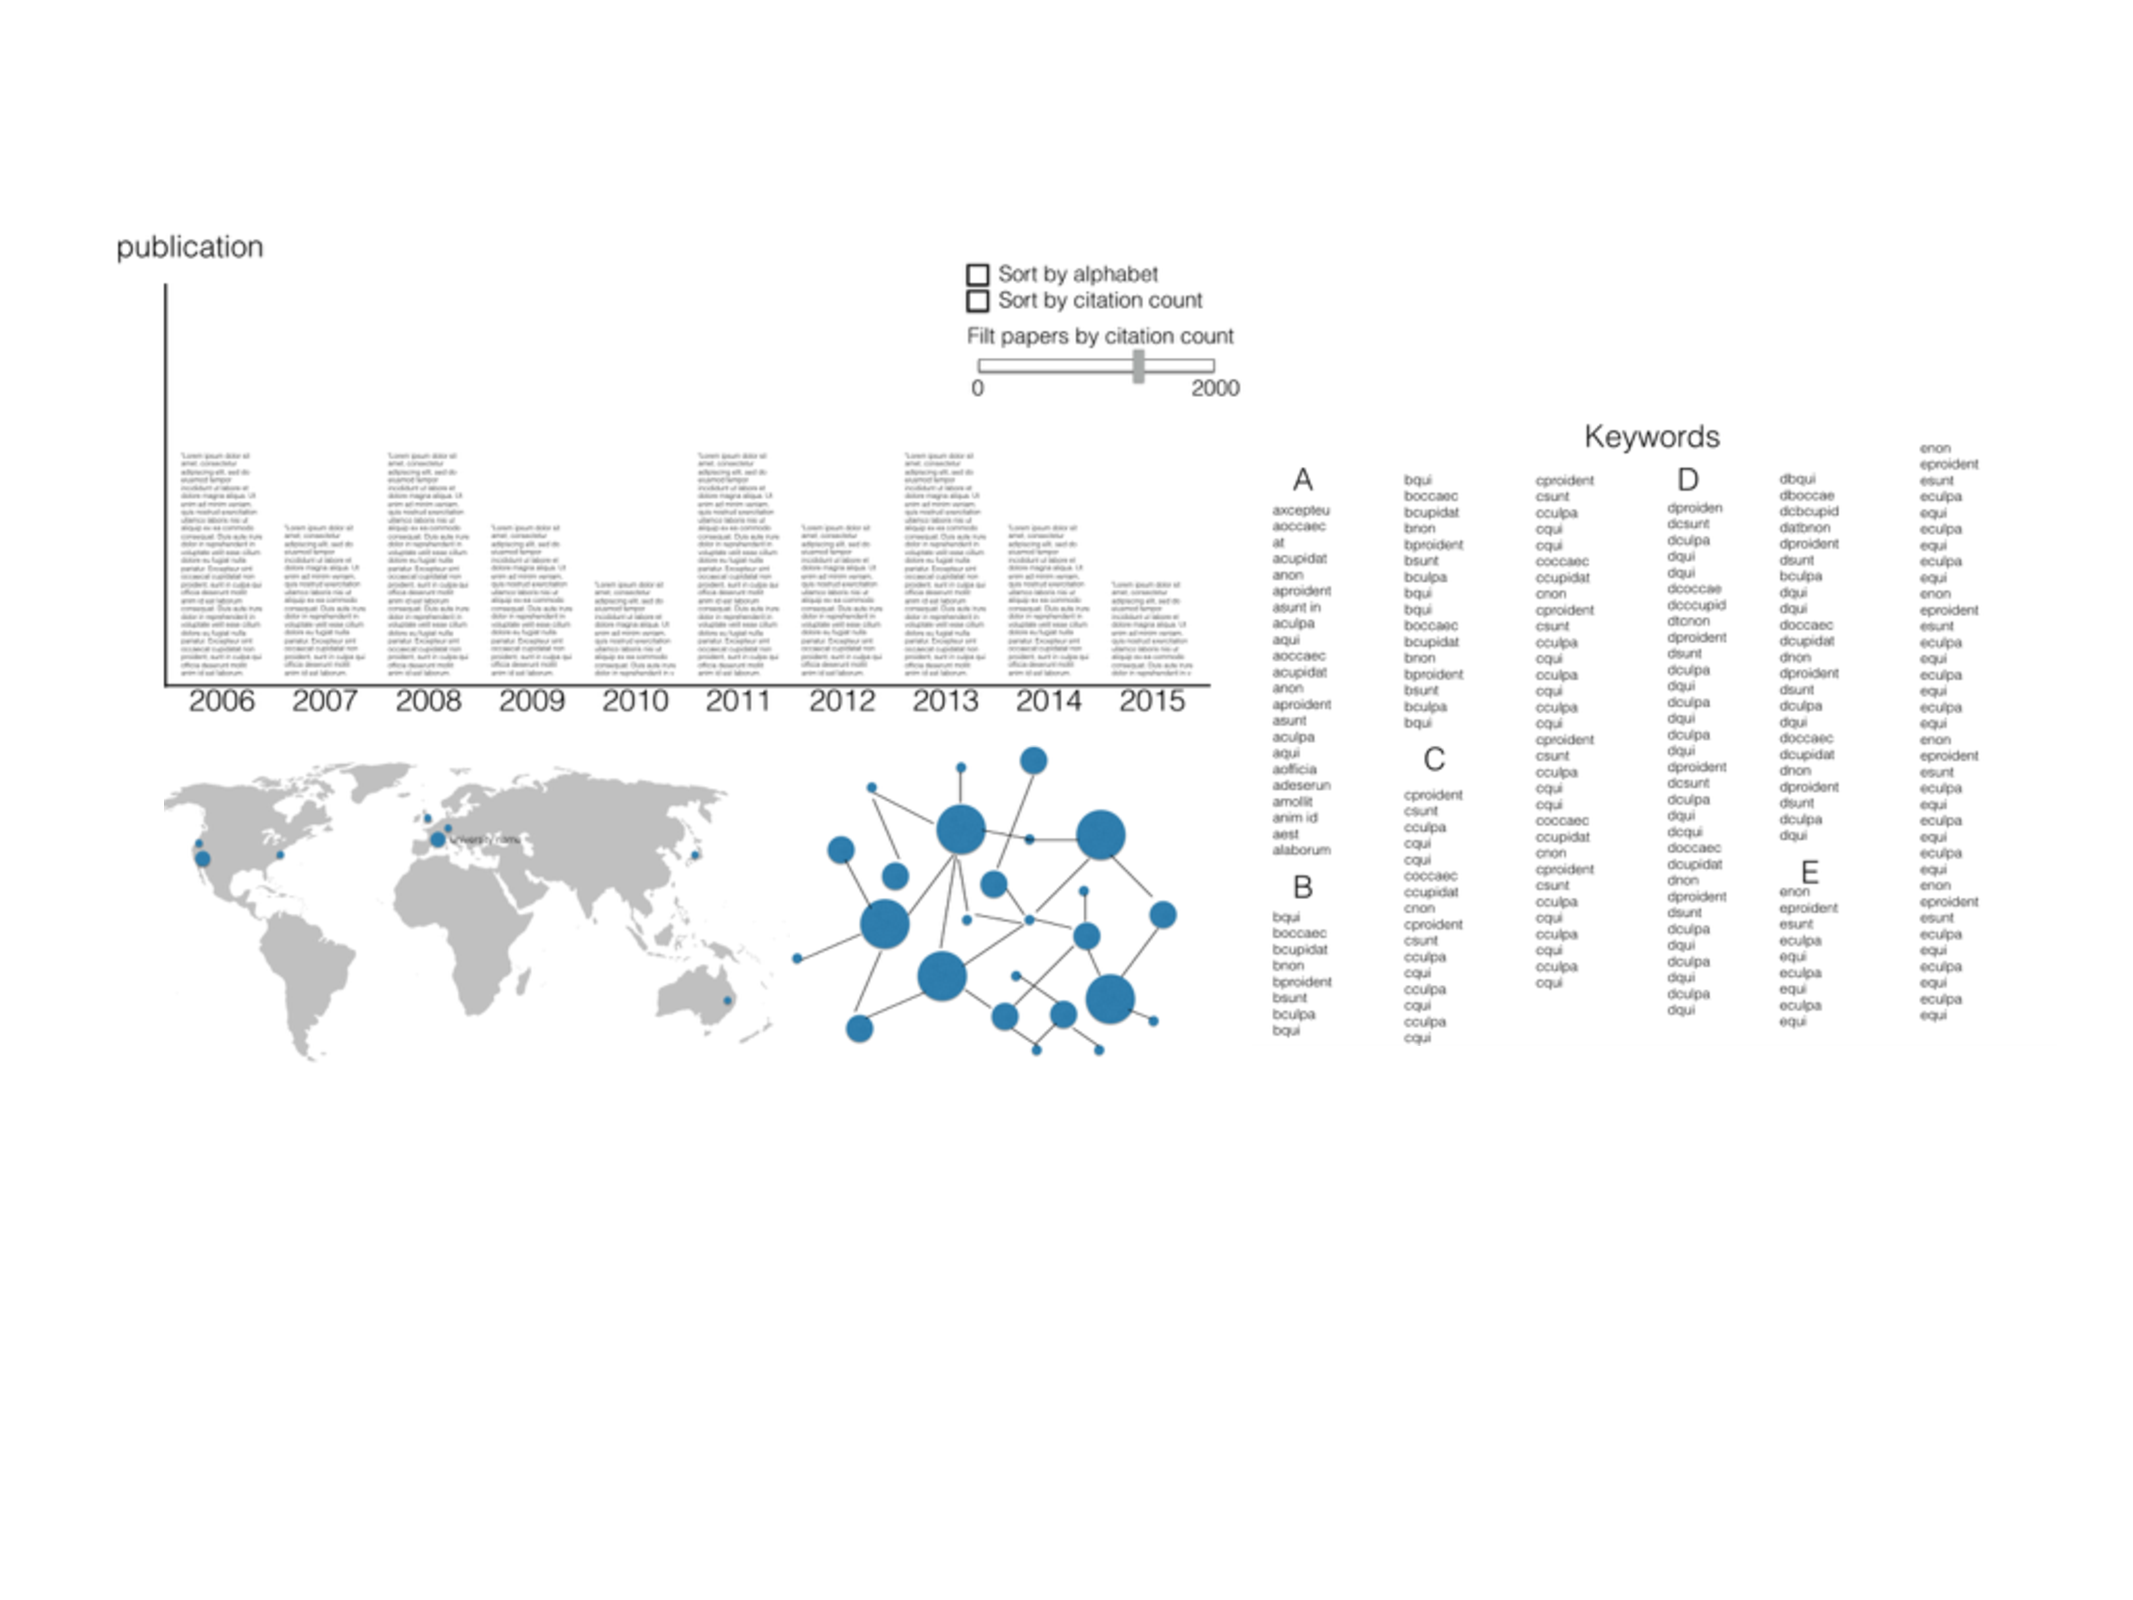
\includegraphics[width=160mm]{visproposalDrawing_page_Part_1.pdf}
    \caption{Overview}
    \label{fig:overview}
\end{figure}

\textbf{Paper view (the main view)}. Here we show all the papers, grouped by year. Each year occupies one column. This view will be wide enough to show about ten years but will be scroll-able horizontally to move the focus to a different period of time. Each paper's title will appear on one row and be click-able. When a paper is clicked on, the papers that this paper cites and the ones that cite it will be highlighted. Moreover, when a paper is mouse over, a pop-up will show the paper's full title, author lists, keywords, and DOI link. A bar will appear right under each paper's title, the length of which is proportional to the paper's number of citations (this is not yet shown in our design sketches). This help the user identify influential papers at a glance.

This whole paper view can be sorted either alphabetically or by citation count. The papers can also be filtered by citation count, to hide papers with lesser impacts. We provide two checkboxes and a slider for these purposes.

\textbf{Institution view}. Here we show a map of all the institutions that have published papers to SIGGRAPH. They will appear as circles on a projected world map. The bigger the circle is, the more publications that institution has in the selected time period. Mousing over an institution will show its name and address. We chose a map for this view because for an institution, the geographical information can be important, for example, to a prospective graduate student looking for a school to apply to. Displaying a large amount of items using circles is also space-conserving.

\textbf{Author view}. In this view we show all paper authors and their collaboration relationships as a node-link diagram. Each author is a node, and two authors are linked if they have written a paper together. Bigger nodes represent more prolific authors, in terms of some metrics such as the H-index. Mousing over an author will show his/her name and affiliations. The reason we chose a node-link diagram for this view is because it highlights quite nicely the clusters between subsets of nodes, and the view is dynamic so it is easier to put any author at the center (for example, when his paper is being selected).

\textbf{Keyword view}. This view acts both as a view and a filter. Here we list all the keywords extracted from all the papers in alphabetical order. Keywords are selectable, and each time a keyword is clicked on, the related keywords are highlighted. This feature is particularly useful when the user clicks on a topic keyword (for example: "global illumination"), and the related keywords show common techniques used to solve problems related to that topic (for example: "path tracing", "radiosity", "photon mapping" which are common methods in graphics to achieve "global illumination"). Two keywords are related if they appear together in many papers. Moreover, selecting a set of keywords will reduce the amount of information shown in the other views, to retain only the papers/authors/institutions that are related to the selected set of keywords. This is useful because the list of papers/authors/institutions can be quite large. Fig \ref{fig:click_keyword} shows an initial design of this idea, where the list of papers was not really filtered by simply highlighted and re-sorted. This feature can be very interesting because a glance at the paper view can tell us the popularity of the current selected set of keywords throughout the years.

\subsection{Final design}
\textbf{Data format}
Because the amount of data we deal with is rather large for a visualization project, initially we thought organizing our data in SQL databases would save storage and data loading time. During the course of implementing the project, however, we have found that our data loading speed is not a problem, even when loading our biggest data files in JSON format (each file is about 2MB each). We therefore forwent the idea of SQL and instead organized our data into multiple JSON files which really simplified the data preparation and loading step.

\begin{figure}[htb!]
    \centering
    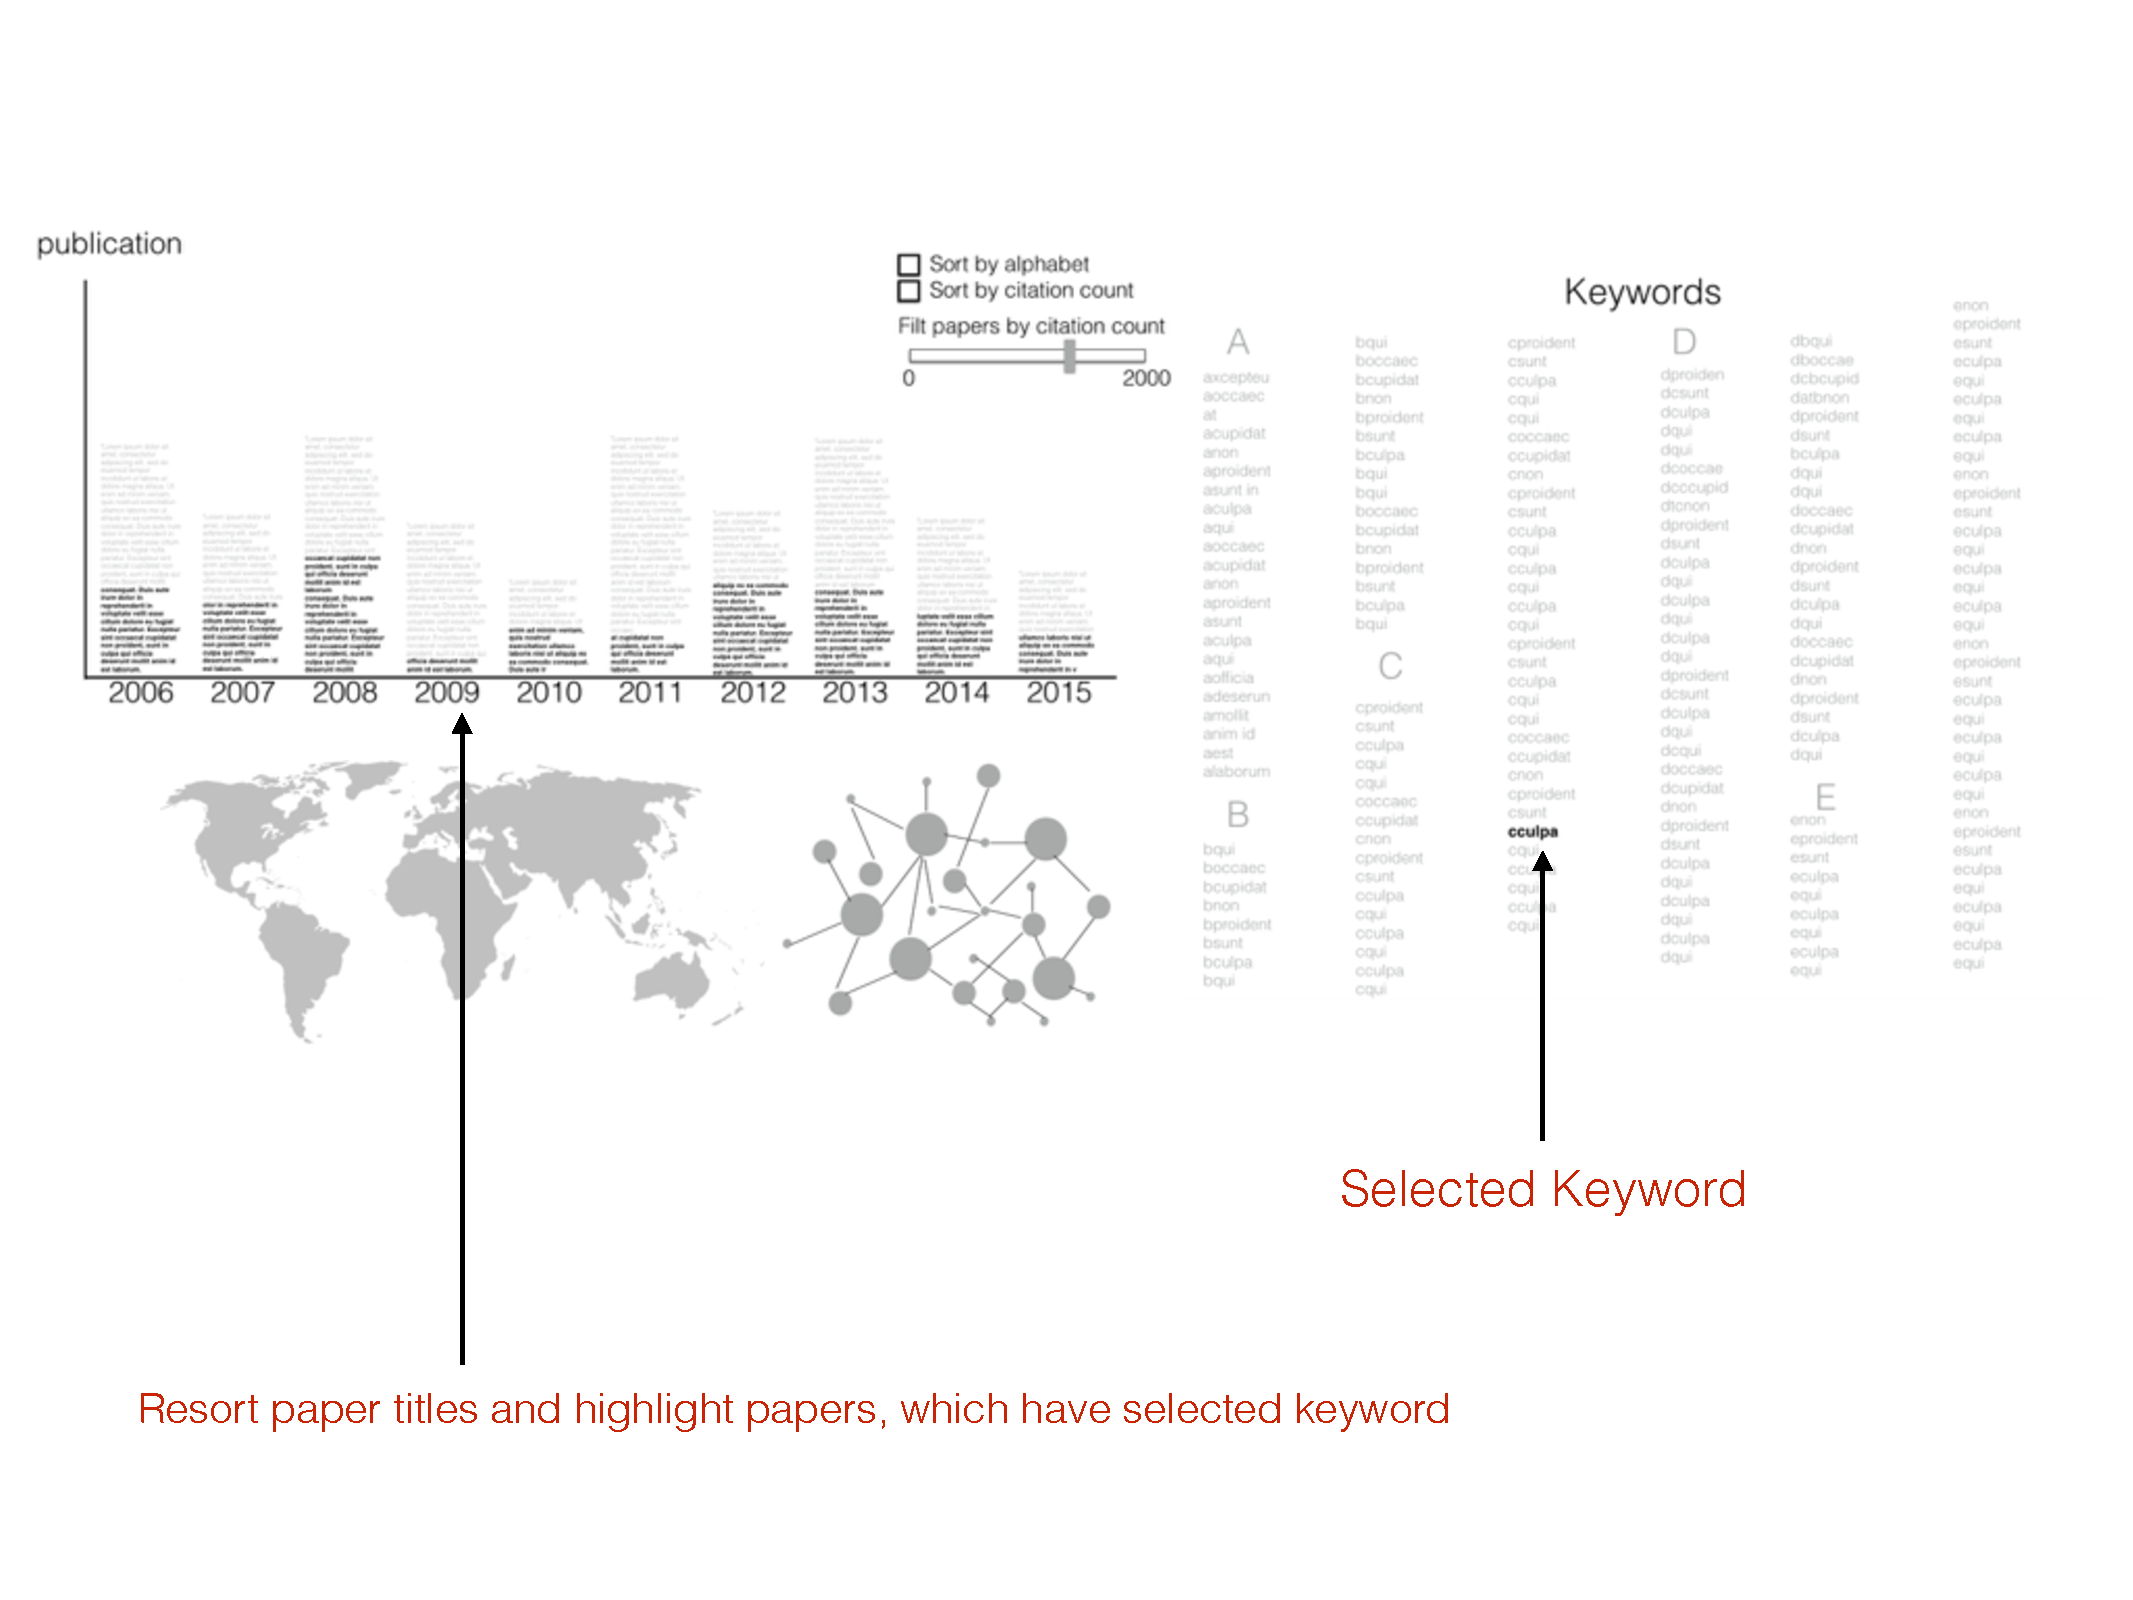
\includegraphics[width=160mm]{visproposalDrawing_page_Part_4.pdf}
    \caption{Keyword filtering}
    \label{fig:click_keyword}
\end{figure}

\textbf{Paper view}
During data processing and implement, we realized that the amount of papers in the each year is quite large, which is about 150 papers per year. As a result, there is no way to arrange the entire paper view, 14 years and 100 papers per year, to one view with proper font size. The initial version of our implementation is shown as Figure~\ref{fig:pv_initial_version}.

\begin{figure}[h]			
	\centering
	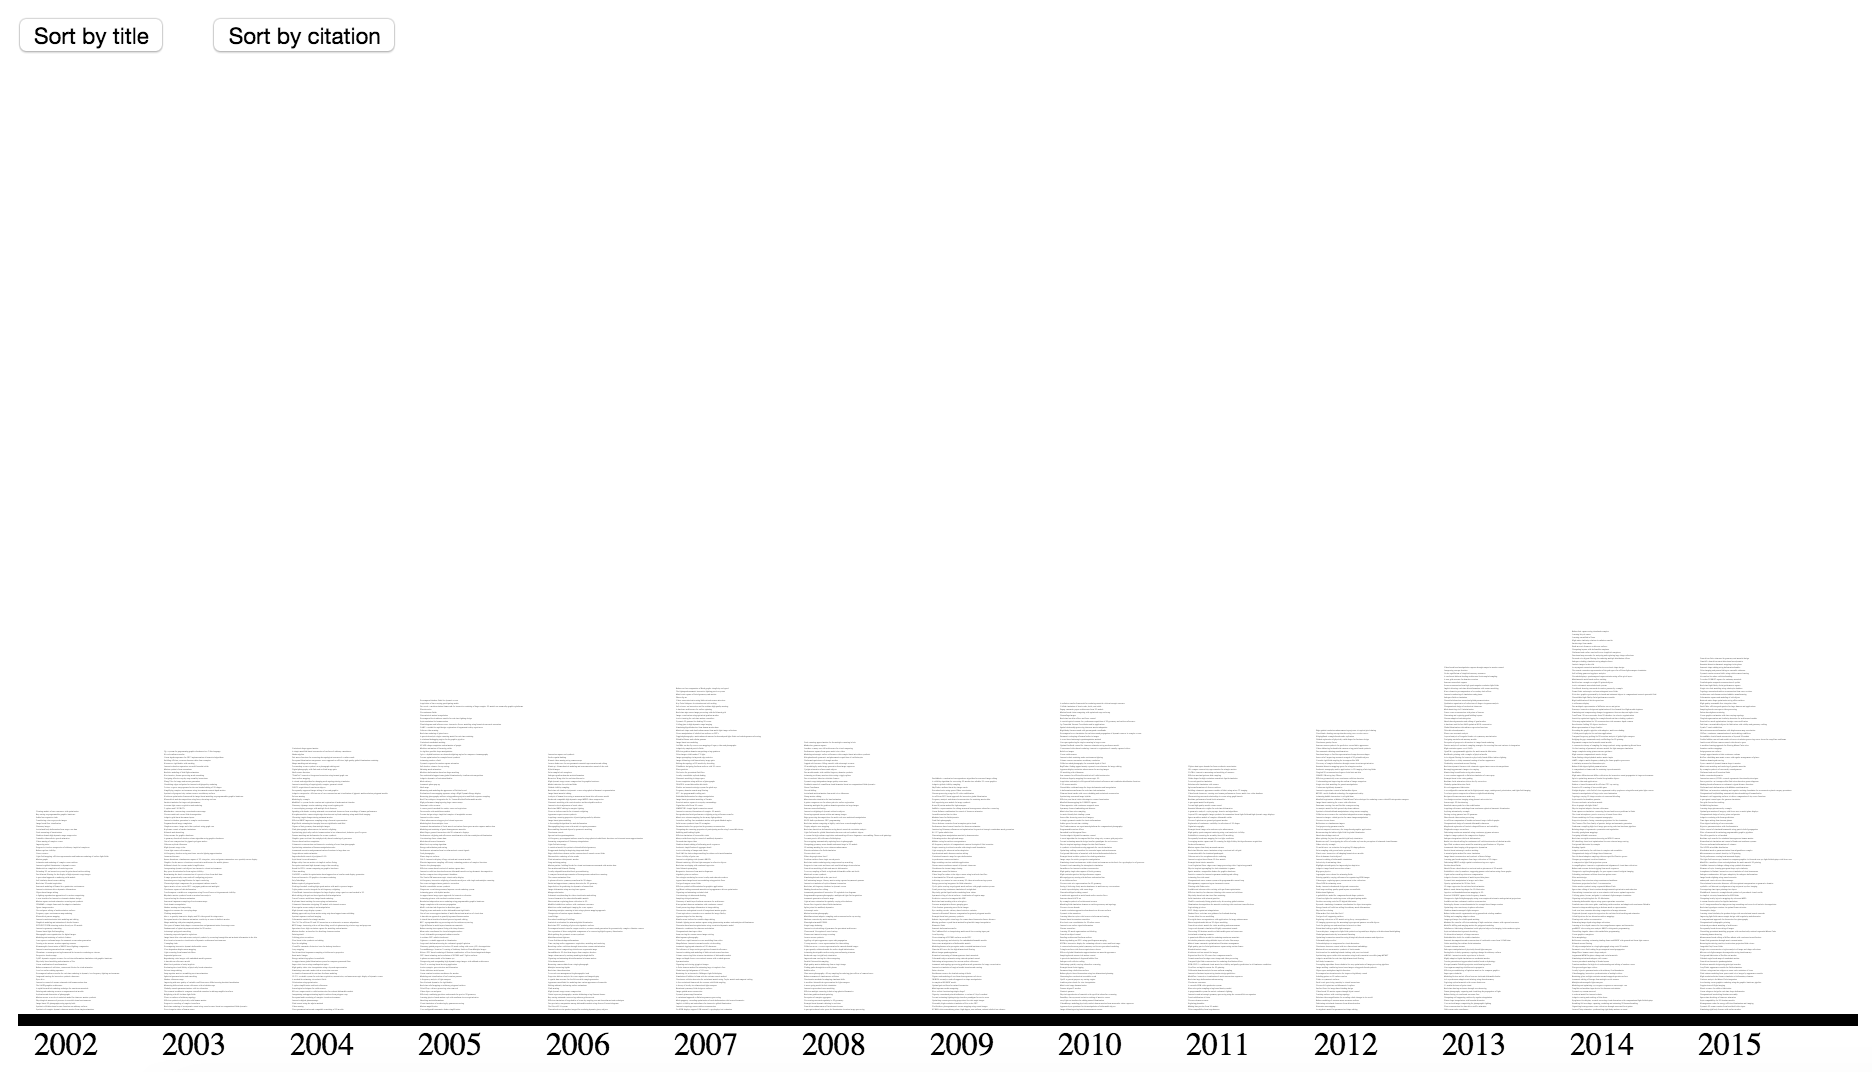
\includegraphics[width=0.7\textwidth]{paper_view_initial_version}
	\caption{The initial version of our paper view implementation}
	\label{fig:pv_initial_version}
\end{figure} 

There are two options to solve this issue. The first one is using zoom in and zoom out to let users explore paper views. We attempt to avoid that method because users may lose the entire view on their mind due to the change blindness. Hence, we added fisheye distortion to enable users to only zoom in texts in a small region as shown in Figure~\ref{fig:pv_fisheye}. However, the fisheye plugin we used is not suitable for zooming in texts. Also, because of the high density of texts, even if we rearrange texts to make it look better, it is still very messy for users to view.

\begin{figure}[ht]			
	\centering
	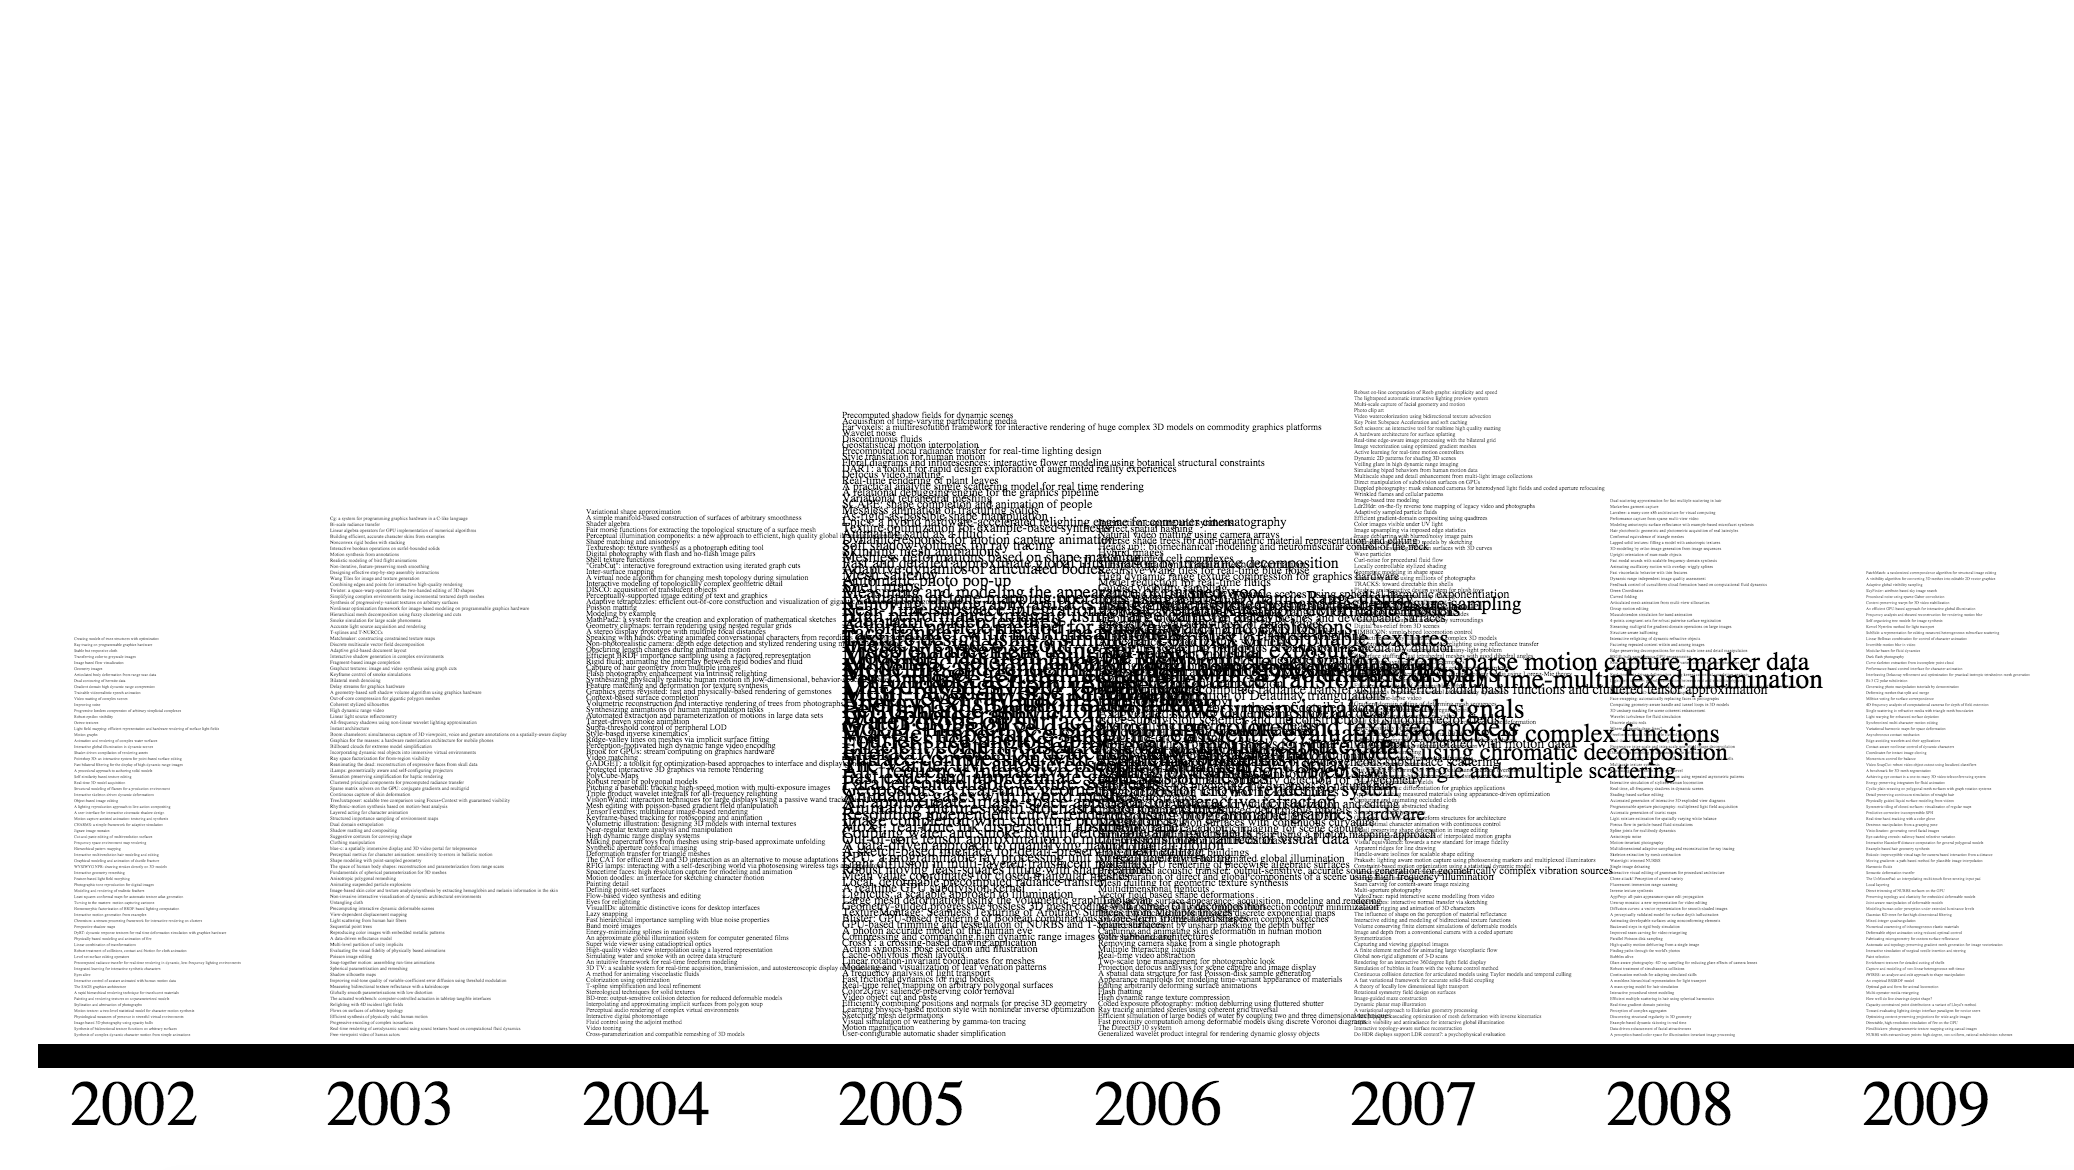
\includegraphics[width=0.7\textwidth]{paper_view_fisheye}
	\caption{Paper view with fish eye}
	\label{fig:pv_fisheye}
\end{figure} 

After that, we decided to add a side bar for the selected year papers as shown in Figure~\ref{fig:pv_side_bar}. When users select one year, the side bar will show all papers in that year and allow users to scroll. We believe this should be the best solution for our issue without zoom in and out. Users can get details as well as overall view at the same time at least.

\begin{figure}[h]			
	\centering
	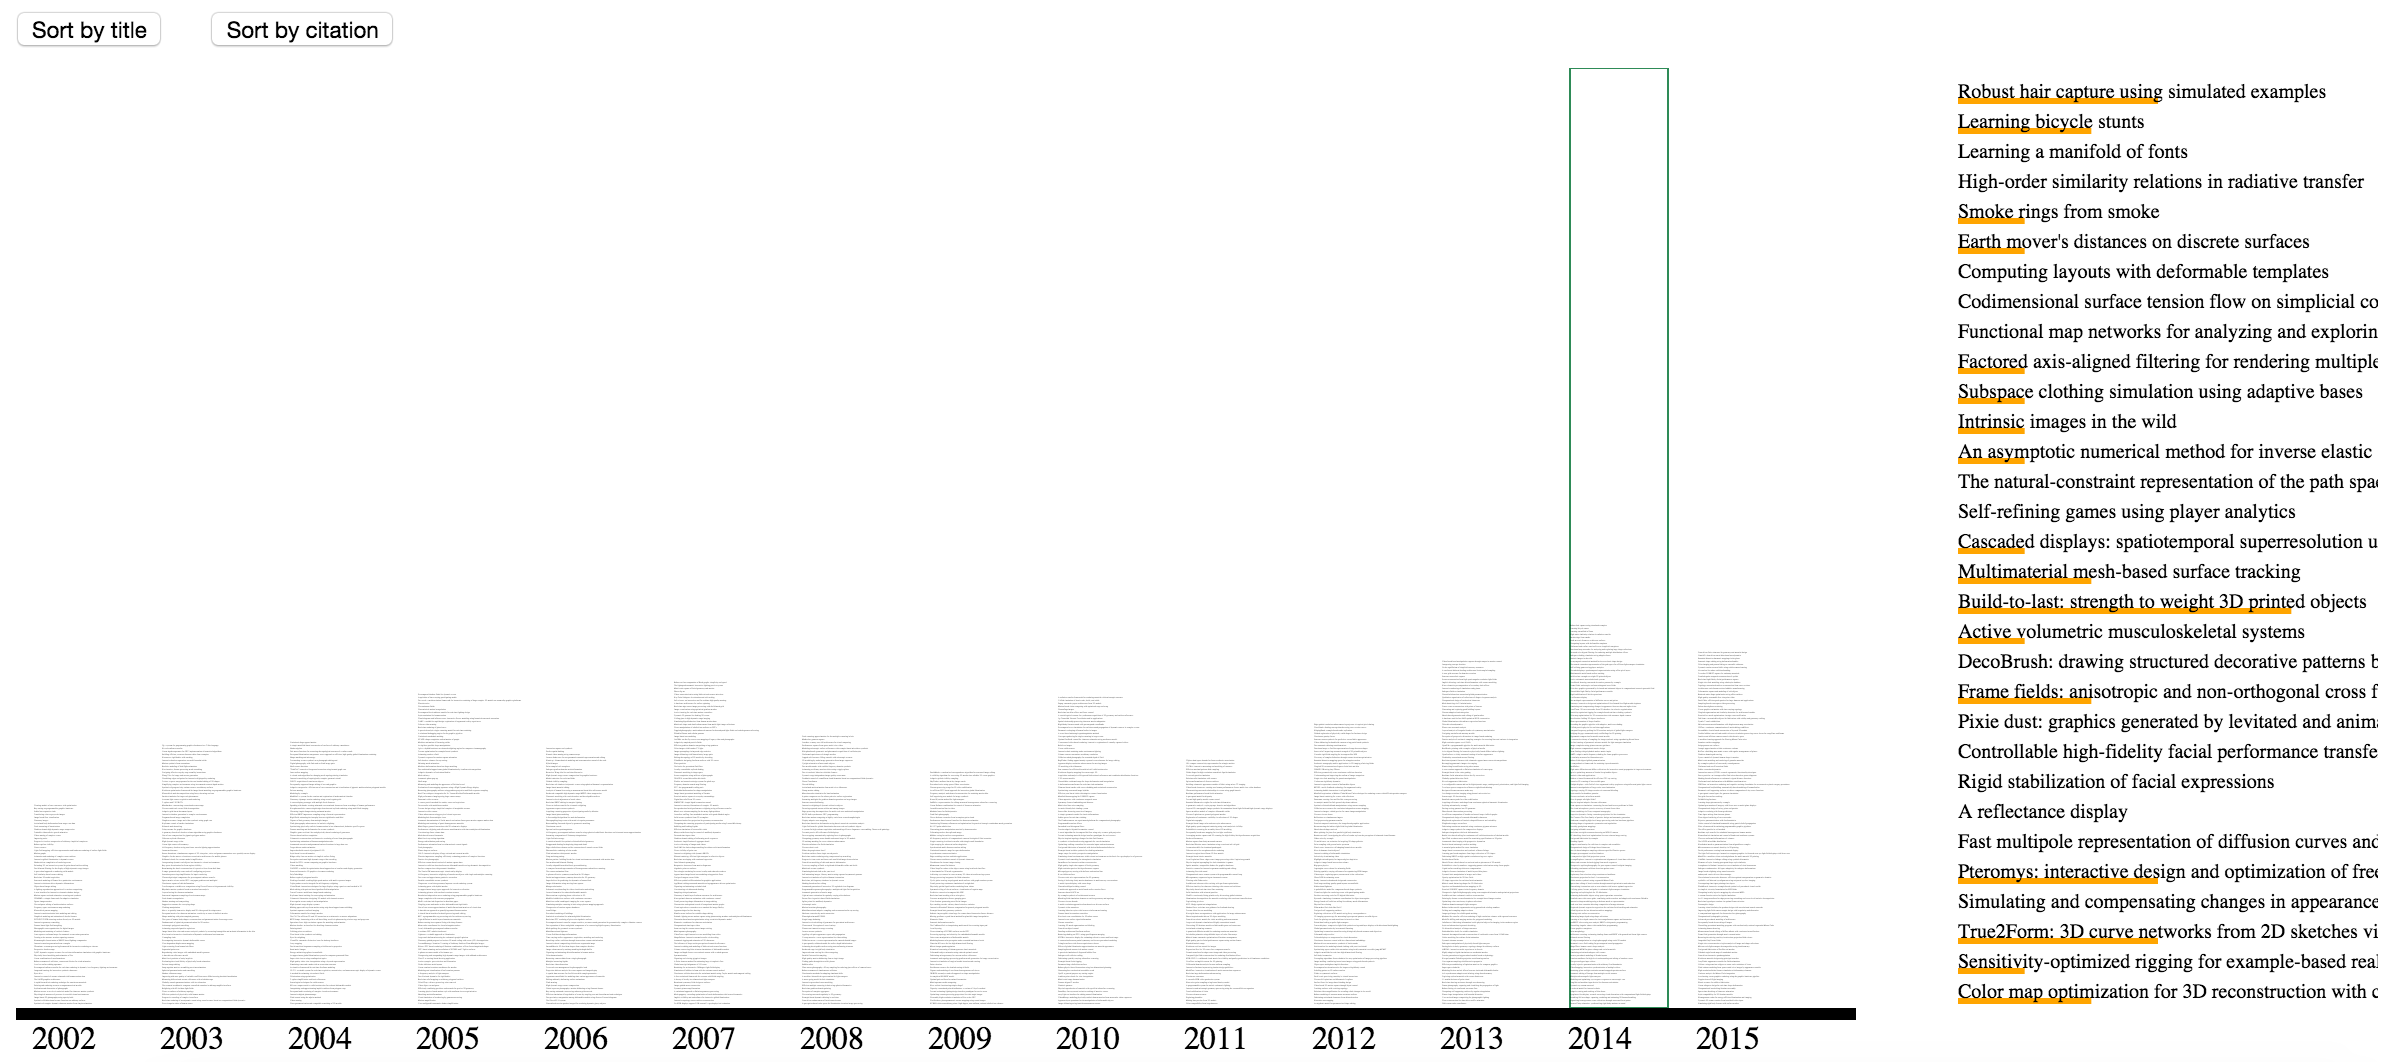
\includegraphics[width=0.7\textwidth]{paper_view_with_side_bar}
	\caption{Paper view with side bar}
	\label{fig:pv_side_bar}
\end{figure} 

However, we meet another question, which is how represent reference and citation relationship between papers in the paper view. As we mentioned before, it is too small to read and we cannot keep our original design as shown in Figure~\ref{fig:overview}. Fortunately, at the worst case, the total amount of reference and citation by one paper is 52. We determined to enlarge the font size of those papers and arrange them by stair shape as shown in Figure~\ref{fig:pv_reference_citation}. We use red and blue to highlight references and cited by papers for now.

\begin{figure}[ht]			
	\centering
	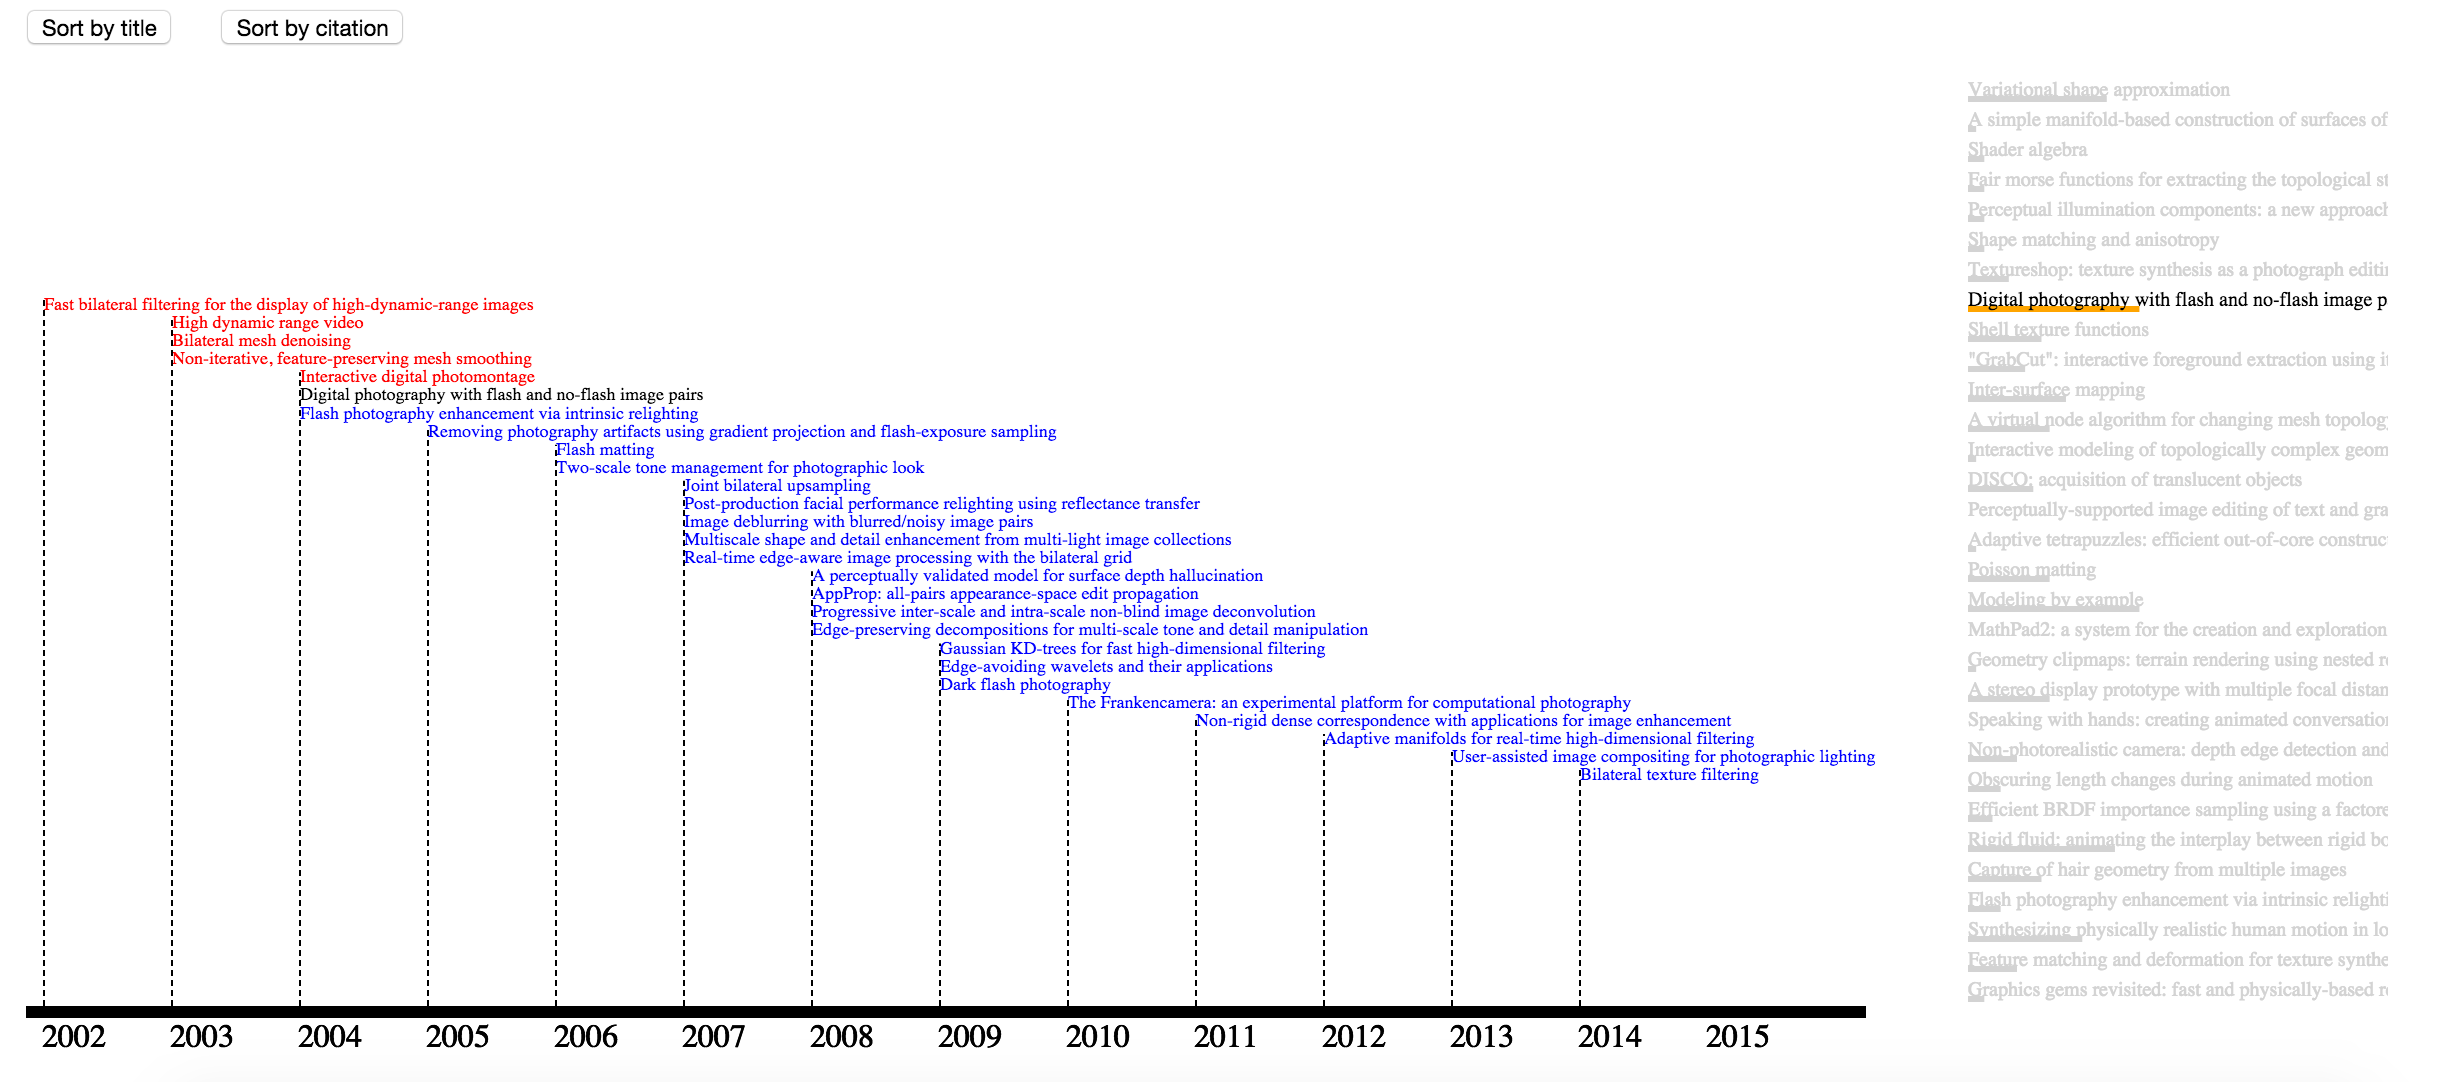
\includegraphics[width=0.7\textwidth]{paper_view_reference_relationship}
	\caption{Paper view with reference and citation for one selected paper}
	\label{fig:pv_reference_citation}
\end{figure} 

Besides that, we also implemented functions, like ``sort title by citation count'' and ``sort title by letter''. More functionalities will be added before final submission.

After milestone 1, we still looked for a better implementation for paper view and attempted to implement our initial design by some alternative ways. Fortunately, we found using scrolling down/up to control zoom in/out is able to provide users a better view control and more freedom to explore the view. Figure~\ref{fig:pv_final} shows our final implementation. Moreover, we add zoom in/out button on the top left of the view to give users hint that the view is zoom-able. 

\begin{figure}[ht]			
	\centering
	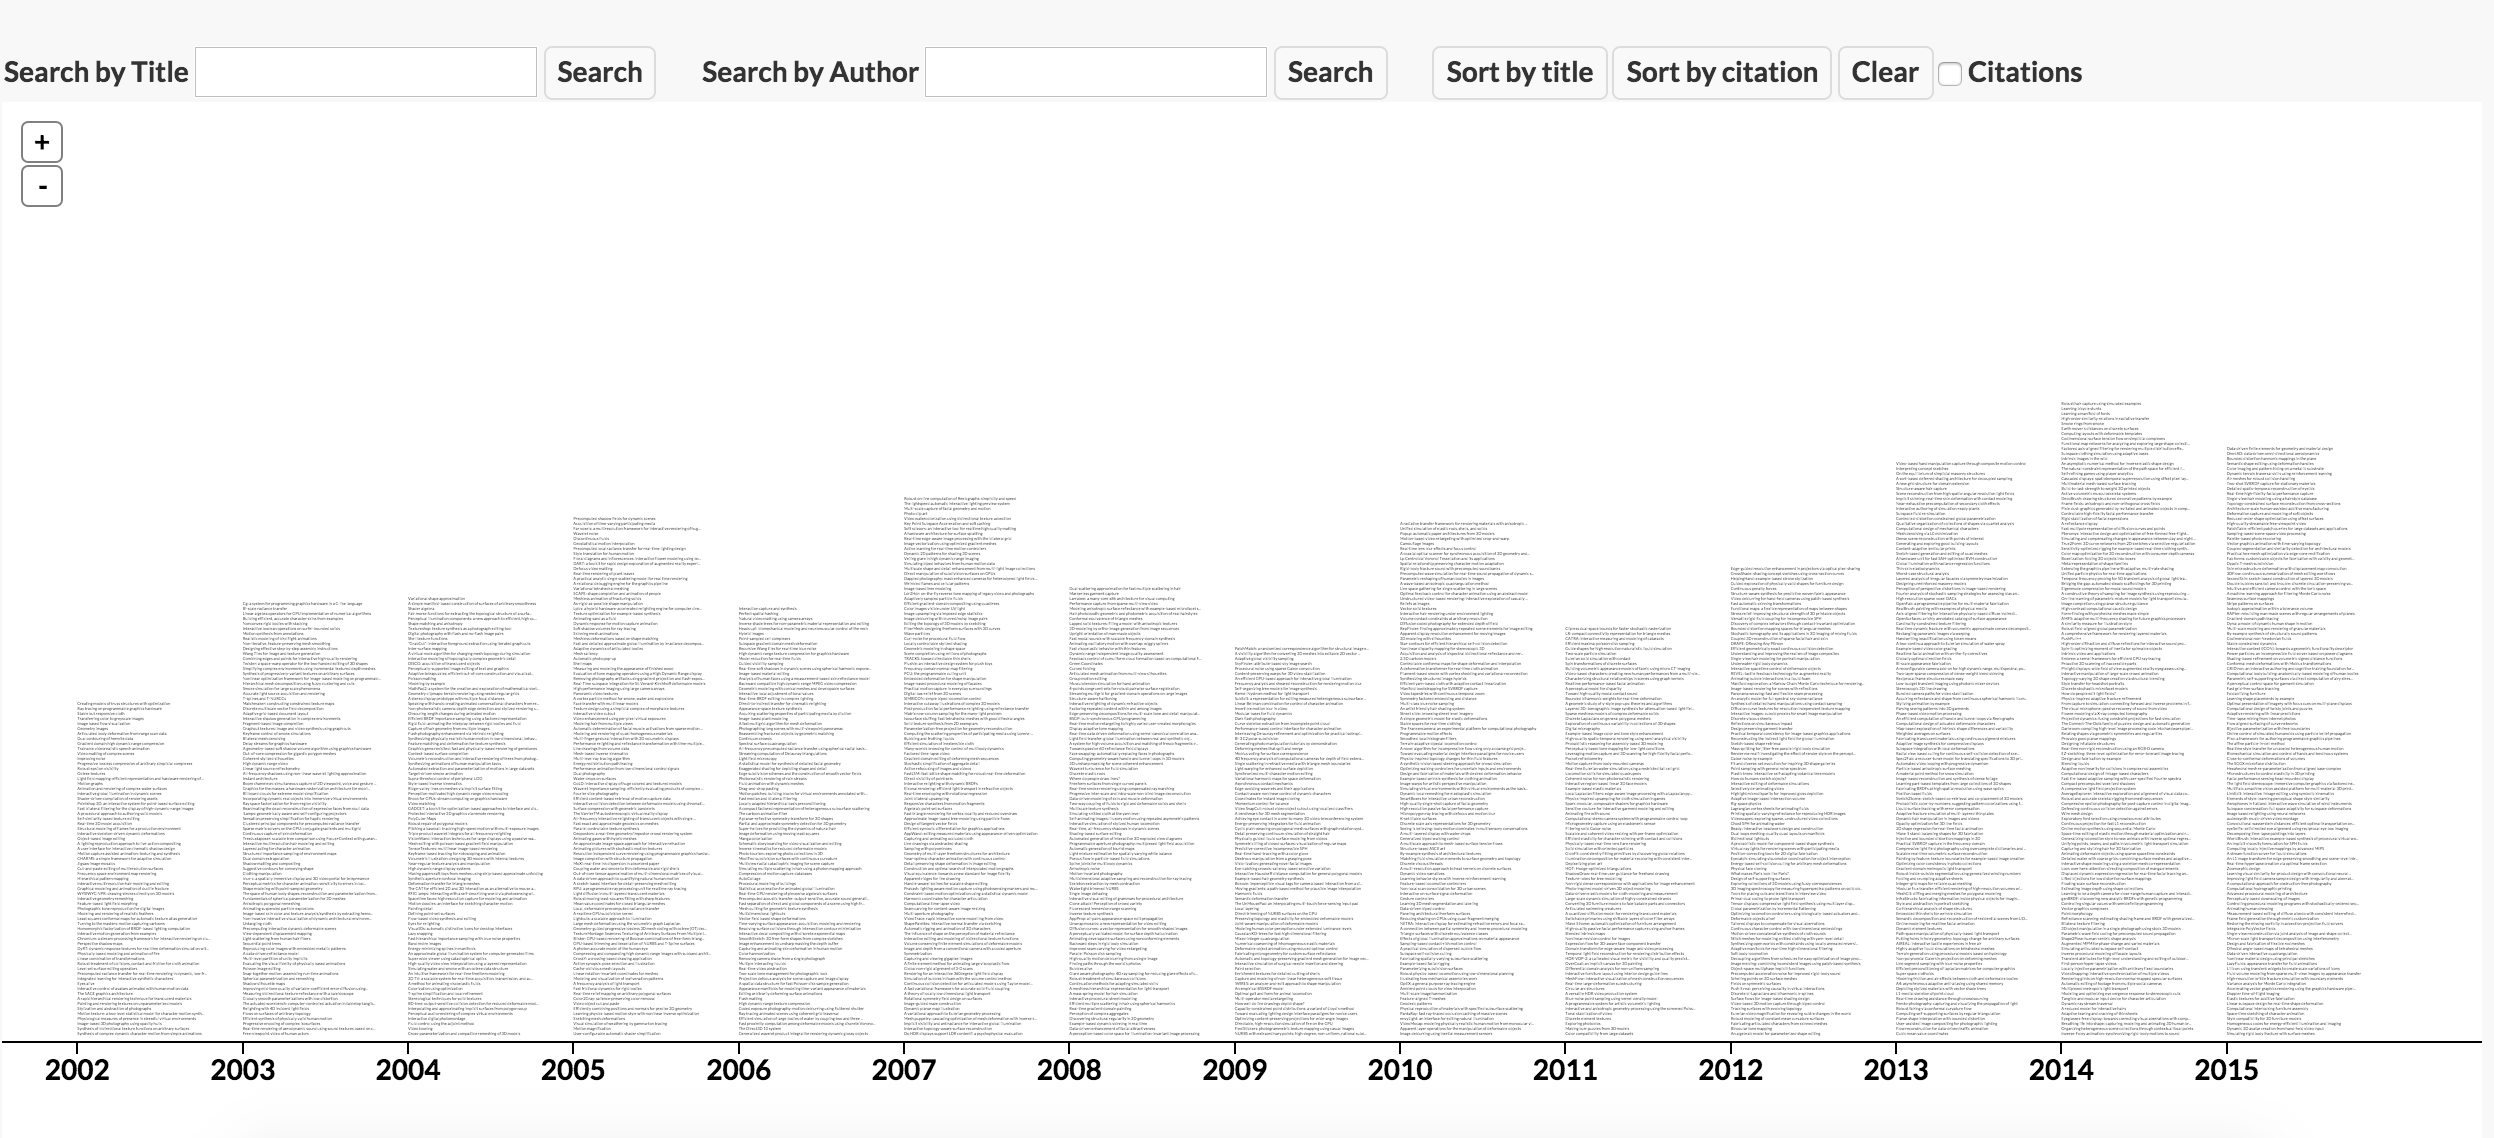
\includegraphics[width=0.7\textwidth]{paper_view_final}
	\caption{Final version of paper view}
	\label{fig:pv_final}
\end{figure} 

\textbf{Paper detail view}
Another benefit for zoom-able paper view is providing more apparently view for user to explore the cited and reference relationship between papers (as shown in Figure~\ref{fig:pv_link}). The main drawback of this alternative is tool-tip may block several papers and cannot contain too many details. Therefore, we add another view for paper details, which include title, authors, abstract, year, keywords, and citation number. Also, in order to give users a brief idea about reference information, we also add a subset paper view here, which only displays the highlighted papers in the paper view. Users can also to use fisheye effect to see titles (as shown in Figure~\ref{fig:pd}).

\begin{figure}[ht]			
	\centering
	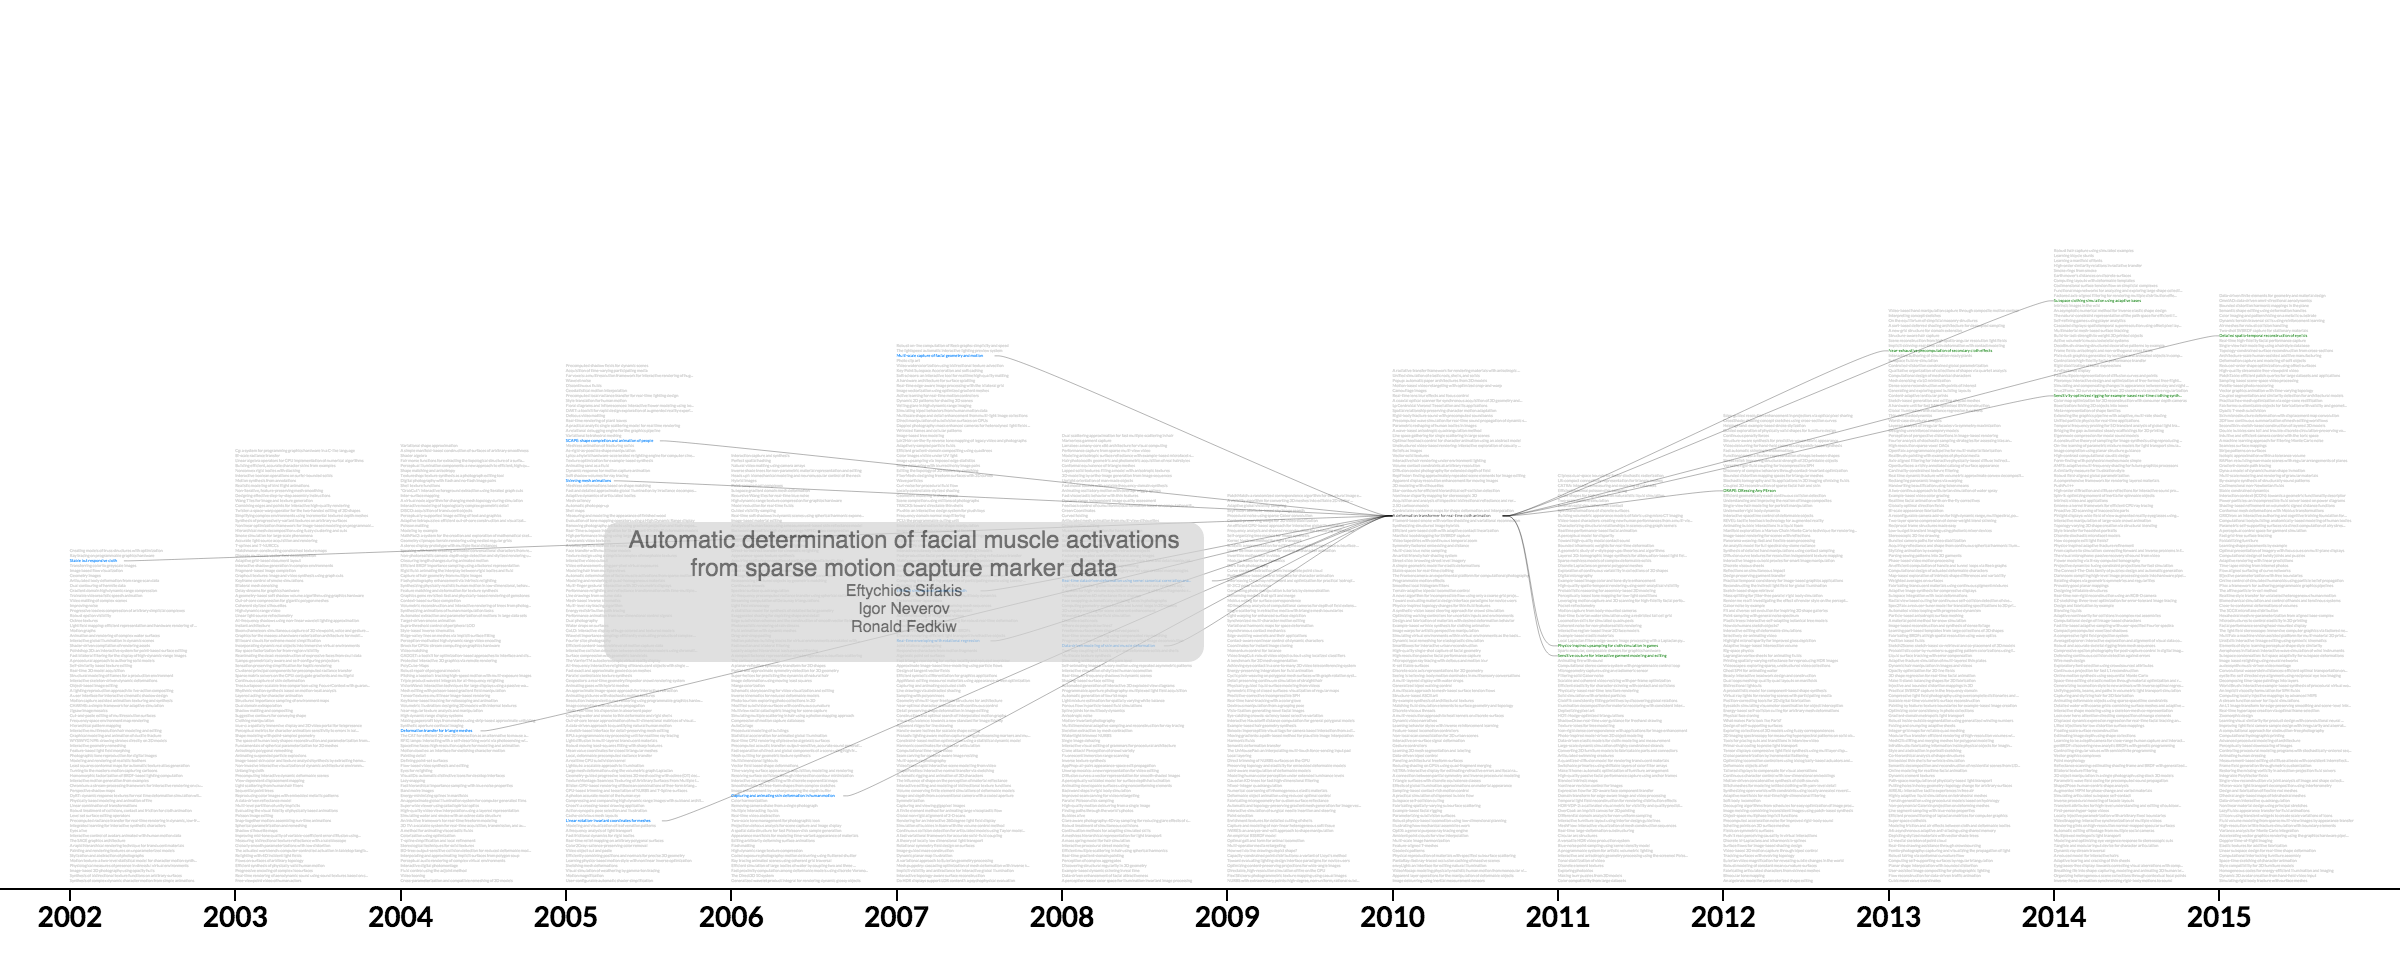
\includegraphics[width=0.7\textwidth]{paper_view_link}
	\caption{Paper view with selected paper}
	\label{fig:pv_link}
\end{figure}

\begin{figure}[ht]			
	\centering
	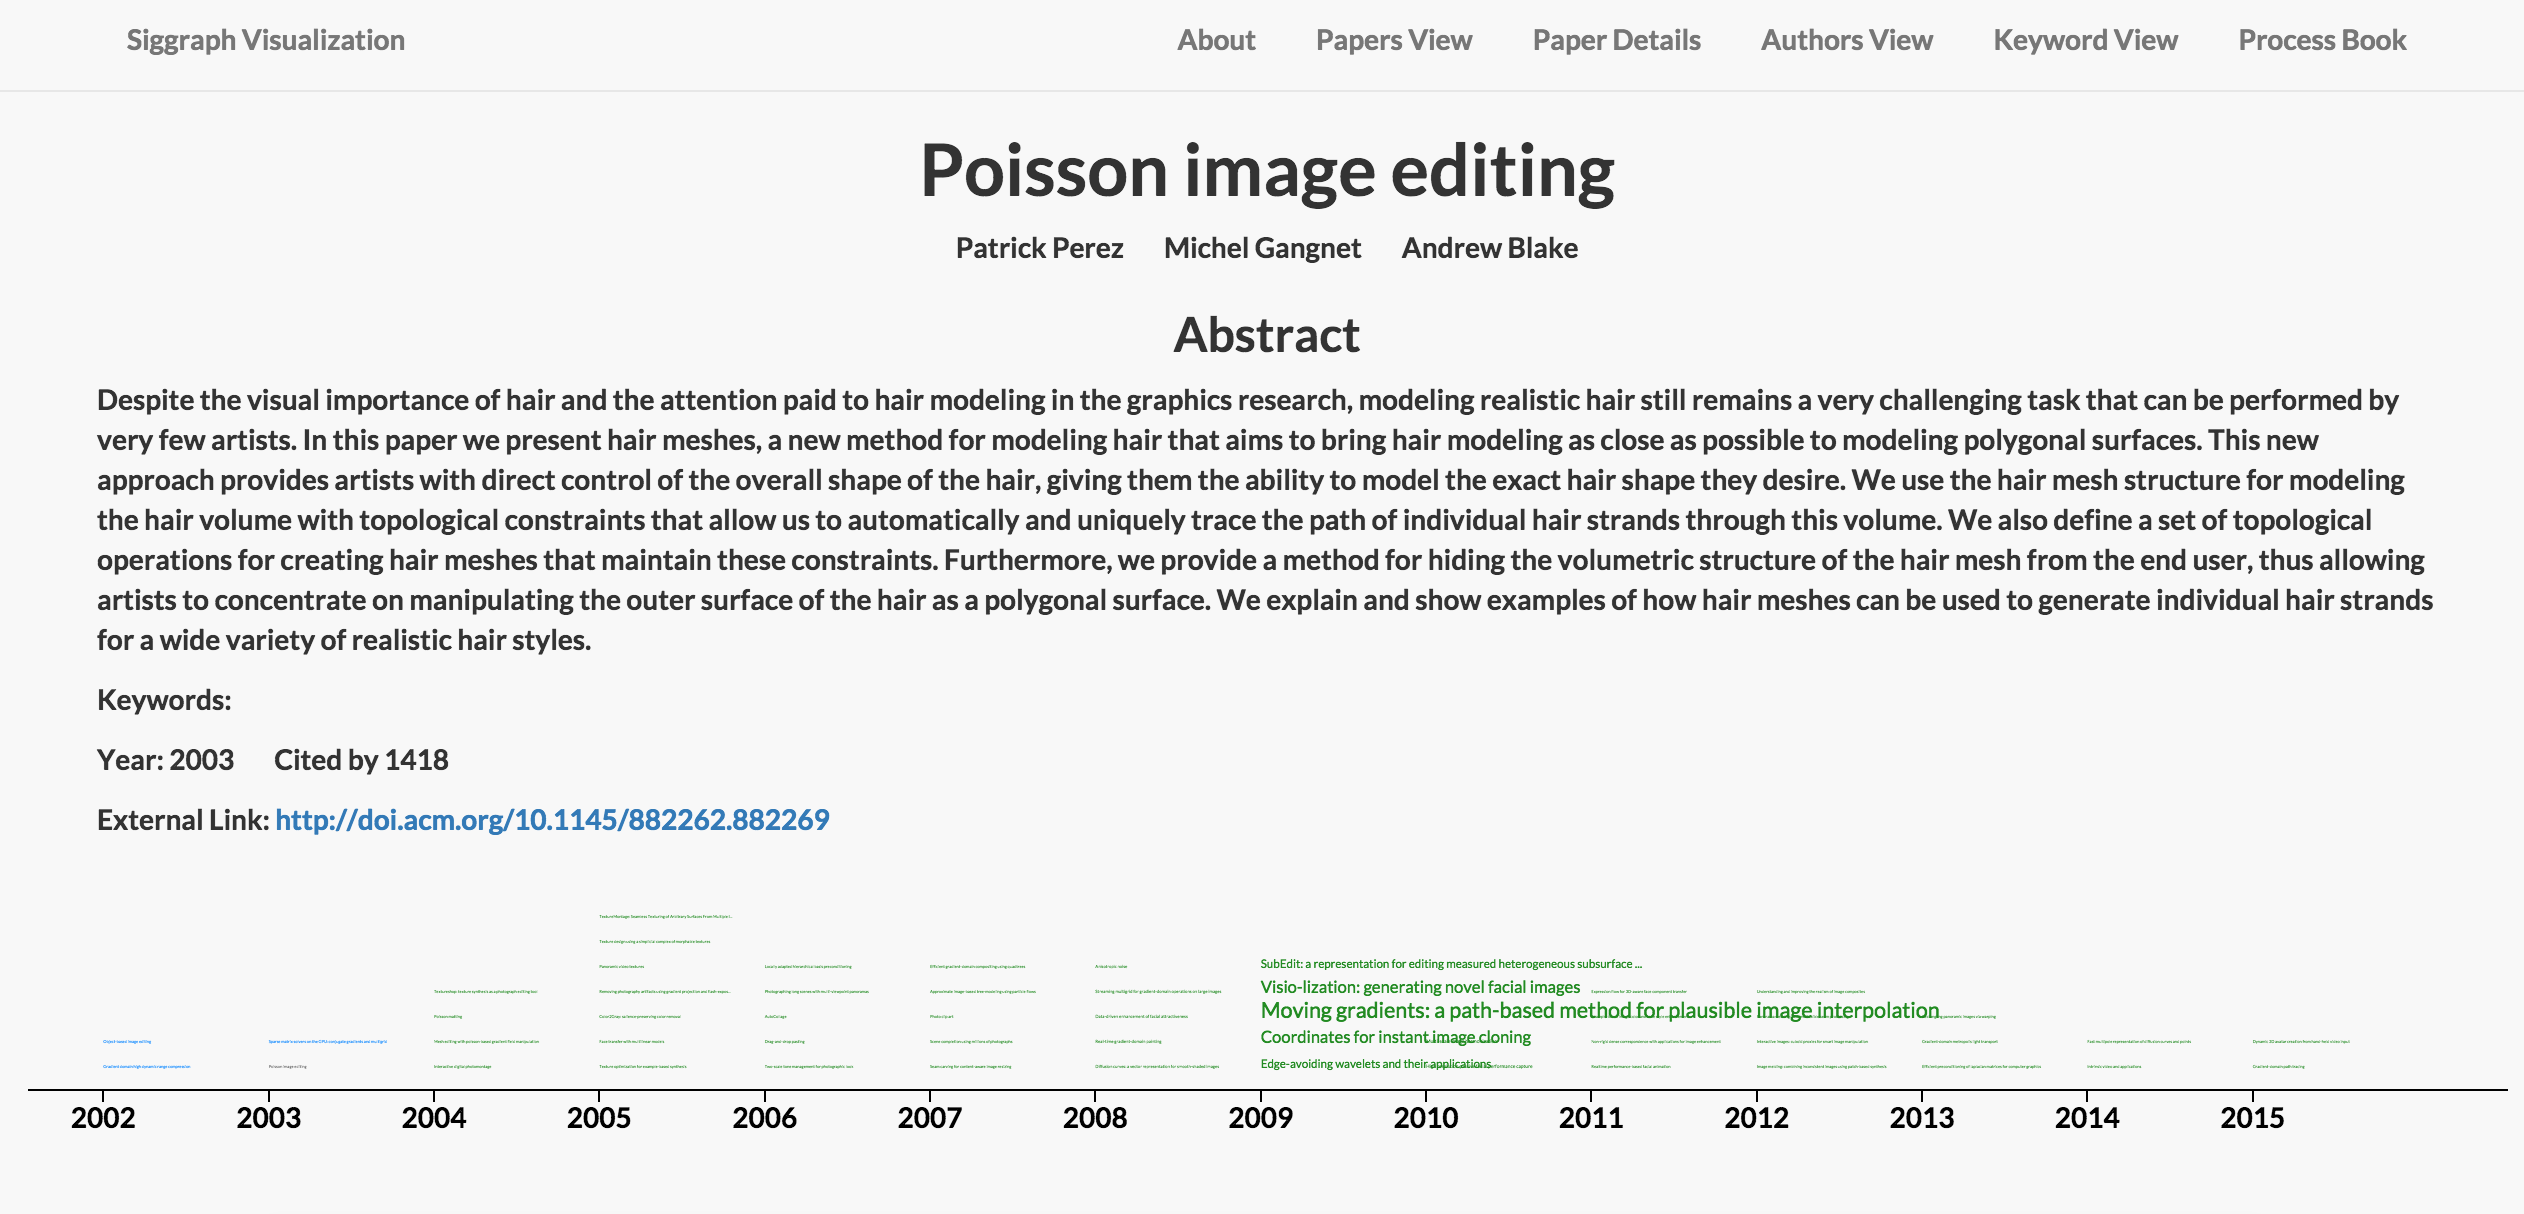
\includegraphics[width=0.7\textwidth]{paper_details}
	\caption{Paper details view}
	\label{fig:pd}
\end{figure}

\begin{figure}[ht]			
    \centering
    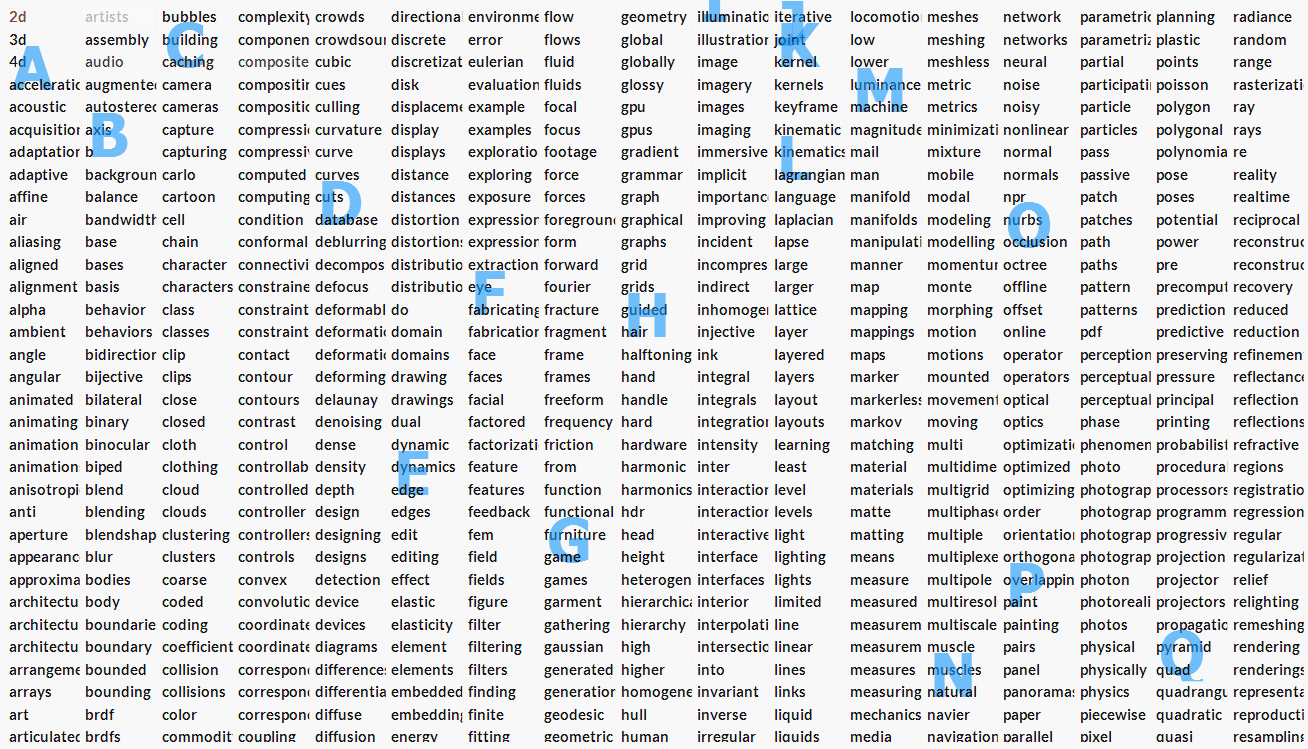
\includegraphics[width=0.7\textwidth]{keyword_view.png}
    \caption{Keyword view}
    \label{fig:kw}
\end{figure}


\textbf{Institution view}
In the meantime, we also realized it is quite difficult to do a university maps view as we promised in the proposal because it is hard to get coordination of universities. So, we decided to get rid of it and add more functionalities to papers view instead, such as searching title. Meanwhile, we can spend more time on keyword view, which we believe is much more useful for users to explore papers. 

\textbf{Author view}
There are about 3500 nodes in the author view, 2200 authors and 1300 papers. It is unreadable if we put all nodes in the view at the same time. Alternatively, we only display the selected paper, its authors, and its authors' publications. Even though it is a much smaller set compared with original one, the view allows user to click and change the selected papers as well. Figure~\ref{fig:av}) demonstrates that mouse-over and tool-tip to show some paper details.

\textbf{Keyword view}
The final design for this view largely follows the initially proposed design. At the time of Milestone 1 we wanted to try out the "bubble" design where the keywords are laid out in circles, using a force-directed method. However, the sheer amount of keywords that we have renders this approach unsuitable. Furthermore, it is better to keep the keywords static (as opposed to making them movable with the mouse), so that the user can rely on his or her memory to locate a keyword quickly. For these reasons, we use a grid layout for the keywords, and provide a search function to help users find the keywords of interest quickly. We also show large characters of the alphabet where that character first appears as the first character of a keyword. These serve as a kind of index into the list of keywords, again, to help with the keyword locating task (Figure \ref{fig:kw}).

\begin{figure}[ht]			
	\centering
	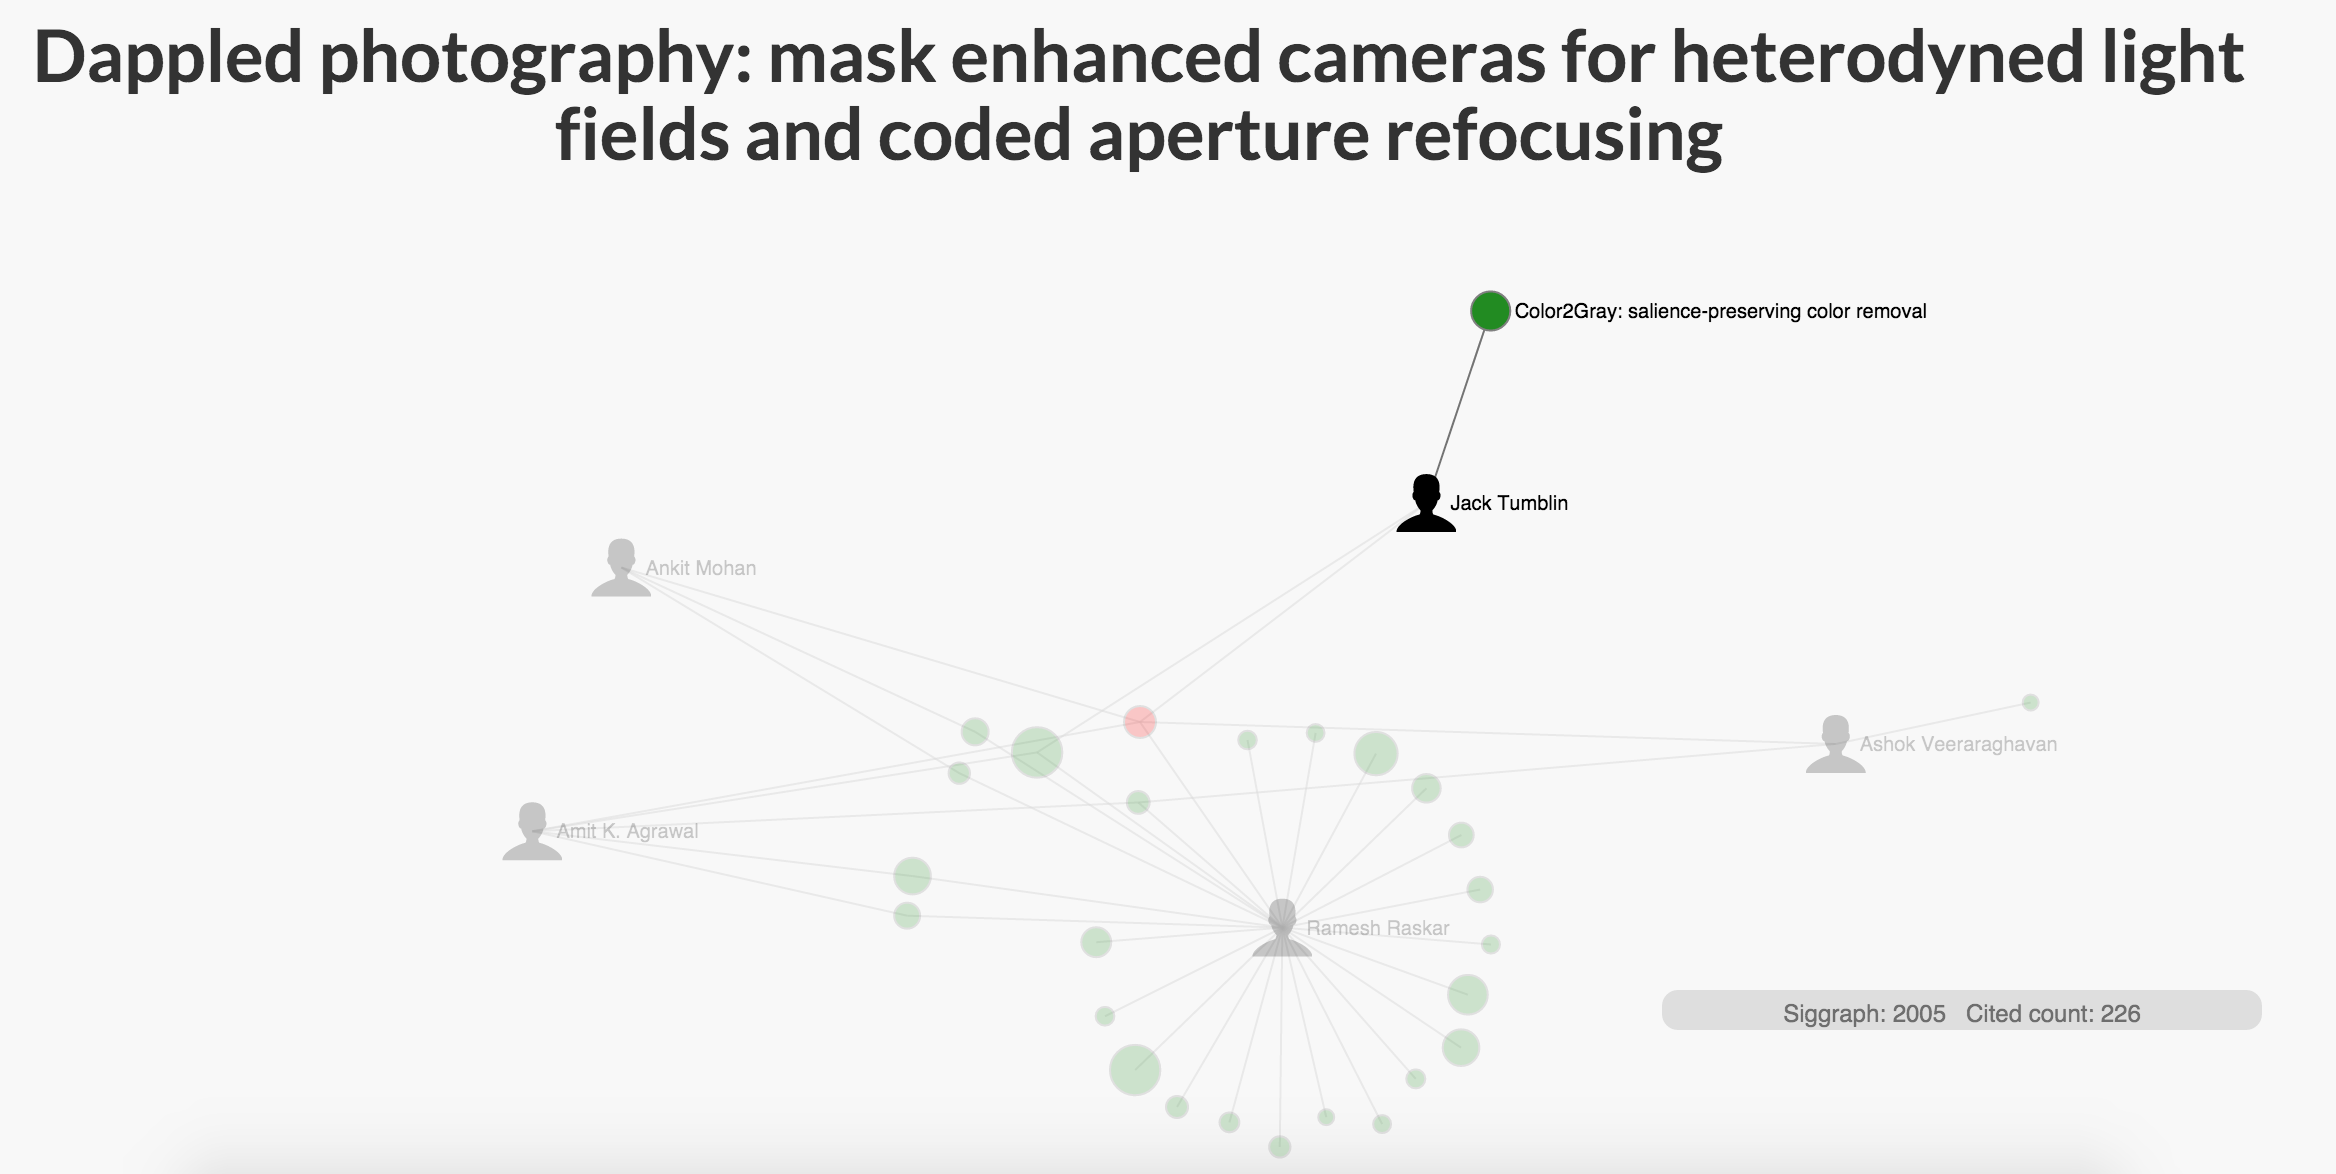
\includegraphics[width=0.7\textwidth]{author_view_with_tooltip}
	\caption{Author view}
	\label{fig:av}
\end{figure} 

\section{Implementation}
Our project includes four view, paper view, paper details view, author view, and keyword view.
\subsection{Paper view}
In paper view, we have we show all the papers, grouped by year. Each year occupies one column. This view is scroll-able horizontally to zoom in/out the view. Zoom in/out button is provided on the left top as well.

Papers' title appears on one row and be click-able. When a paper is clicked on, the papers that this paper cites and the ones that cite it will be highlighted with different color. Curved links are display to show the relationship between papers. Moreover, when a paper is mouse over, a pop-up will show the paper's full title, author lists. 

This whole paper view can be sorted either alphabetically or by citation count. We provide a checkbox to display/hide citation count bar. The citation bar appears right under each paper's title, the length of which is proportional to the paper's number of citations and scaled within the year, because it is unfair to compare two papers published in different years. This help the user identify influential papers at a glance.

There are also two search buttons, which allows user to search author name or paper title. If more than papers are returned, all of them will be highlighted as black. If only return one result, the result will set as selected paper and showing its reference.

Once paper is selected, paper details and author view will be updated correspondingly based on the selection.

\subsection{Paper details view}
Paper view shows all details about the selected paper, including title, authors, abstract, keywords, cited count, year, and its external link, which points to ACM web-site.

Keywords are click-able. Once keywords is clicked, it will be set as "selected" and update keyword view.

Also, in order to give users a brief idea about reference information, a subset paper view is added here, which only displays the highlighted papers in the paper view. Titles here also can be enlarged when mouse over it.

\subsection{Author view}

Author view only displays the selected paper, its authors, and its authors' publications. Each green circle represents one paper and is scaled by its cited count.  Even though it is a much smaller set compared with original one, the view allows user to click and change the selected papers with transition. 

When users mouse-over it, a tool-tip will show on the right bottom to show published year and cited count. In the mean time, other unconnected nodes will be transparent so to highlight mouse-over-ed paper and its author or  mouse-over-ed author and all his/her publications.

\subsection{Keyword view}
In this view we display all the keywords extracted from our paper database. Since the number of keywords are large (we have nearly a thousand keywords), we opted for a simple view where the keywords are sorted in alphabetical order and shown in a grid. Some keywords are long and will thus be truncated in the view, but will be shown in full when the user moves the mouse over. We achieved this by fading out the two adjacent keywords. The list of keywords can be filtered using a search box (irrelevant keywords will be grayed out). Keywords are clickable. When a keyword is clicked on, it will be highlighted, together with all its related keywords. Two keywords are related if they appear together in more than one papers (Figure \ref{fig:kw_selected}).

\begin{figure}[ht]			
    \centering
    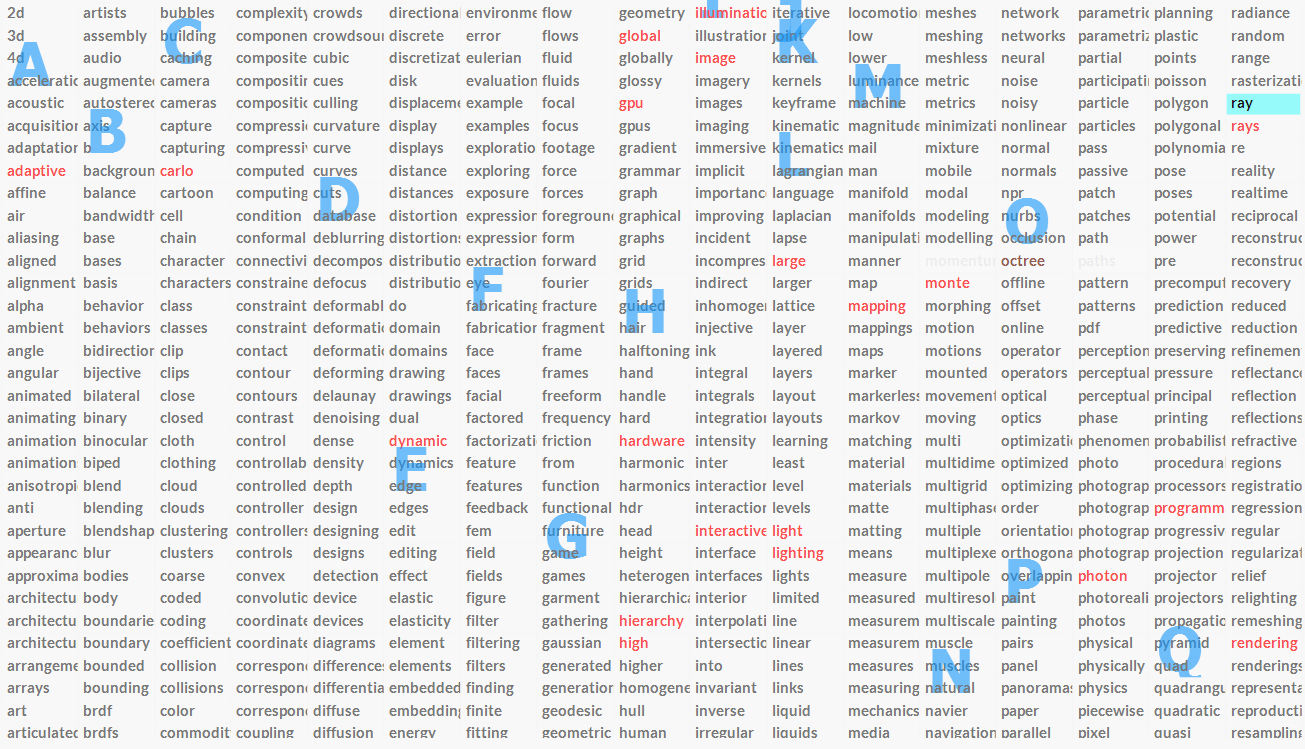
\includegraphics[width=0.7\textwidth]{keyword_view_selected.png}
    \caption{Keyword view with a keyword selected}
    \label{fig:kw_selected}
\end{figure}

Selecting a set of keywords will have an effect on the paper view. Papers having all the selected keywords will be highlighted. This is very useful for exploration of the paper database based on keywords.


\section{Evaluation}
In this section, we demonstrate a typical usage scenario of our tool. Let's say the user is interested in all papers that address the problem of "global illumination". This is one of the fundamental, long-standing problems in computer graphics.

We start by looking at the keywords and clicking on "global" and "illumination". These keywords can be found by either starting the search at the letter "G" and "I", or by using the search textbox. Once these two keywords are clicked on, other related keywords are also highlighted (Figure \ref{fig:global_illumination_selected}).

\begin{figure}[ht]			
    \centering
    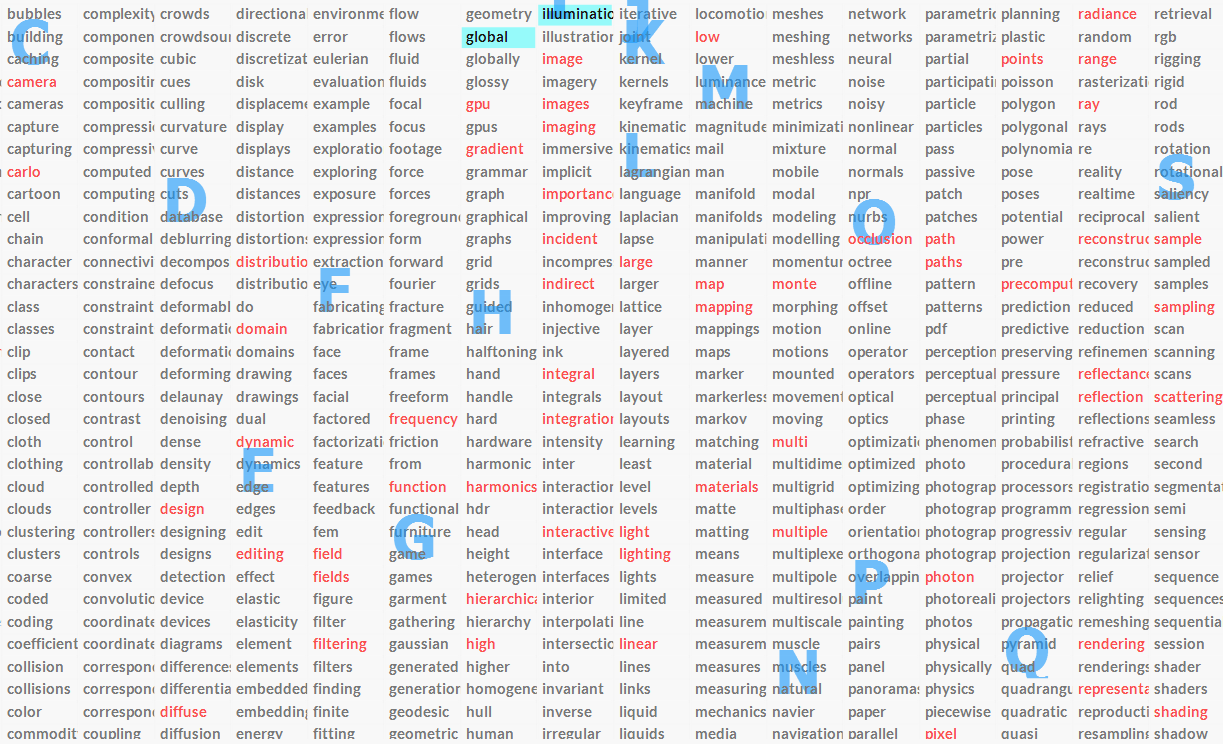
\includegraphics[width=0.7\textwidth]{global_illumination_clicked.png}
    \caption{"global" and "illumination" keywords selected}
    \label{fig:global_illumination_selected}
\end{figure}

In the paper view, papers with both the keywords are highlighted (Figure \ref{fig:global_illumination_papers}).

\begin{figure}[ht]			
    \centering
    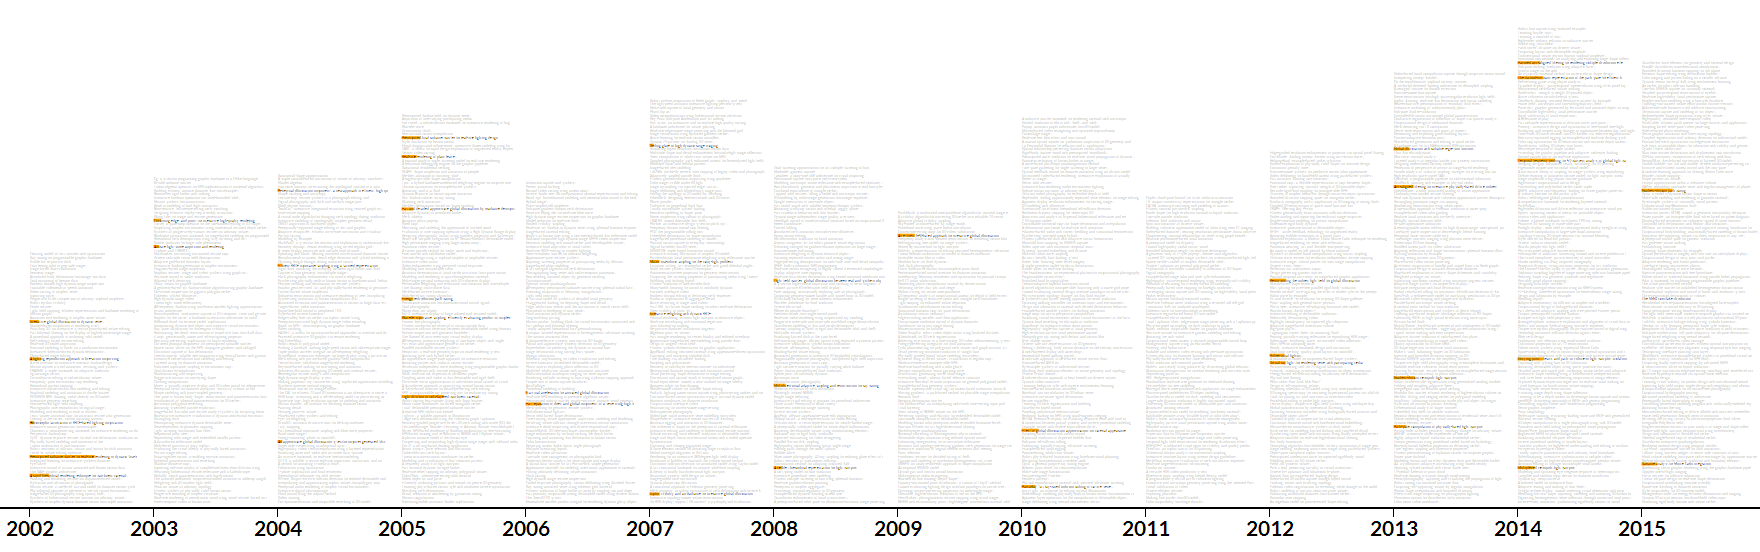
\includegraphics[width=0.7\textwidth]{global_illumination_papers.png}
    \caption{Papers with both keywords: "global" and "illumination" keywords selected}
    \label{fig:global_illumination_papers}
\end{figure}

There are two highlighted papers in 2015, one of them having significantly more citations than the other. Since we are interested in the state-of-the-art research, we click on the one in 2015 with more citations. This paper is called "Gradient domain path tracing" (Figure \ref{fig:gradient_domain_path_tracing_paper_selected}).

\begin{figure}[ht]			
    \centering
    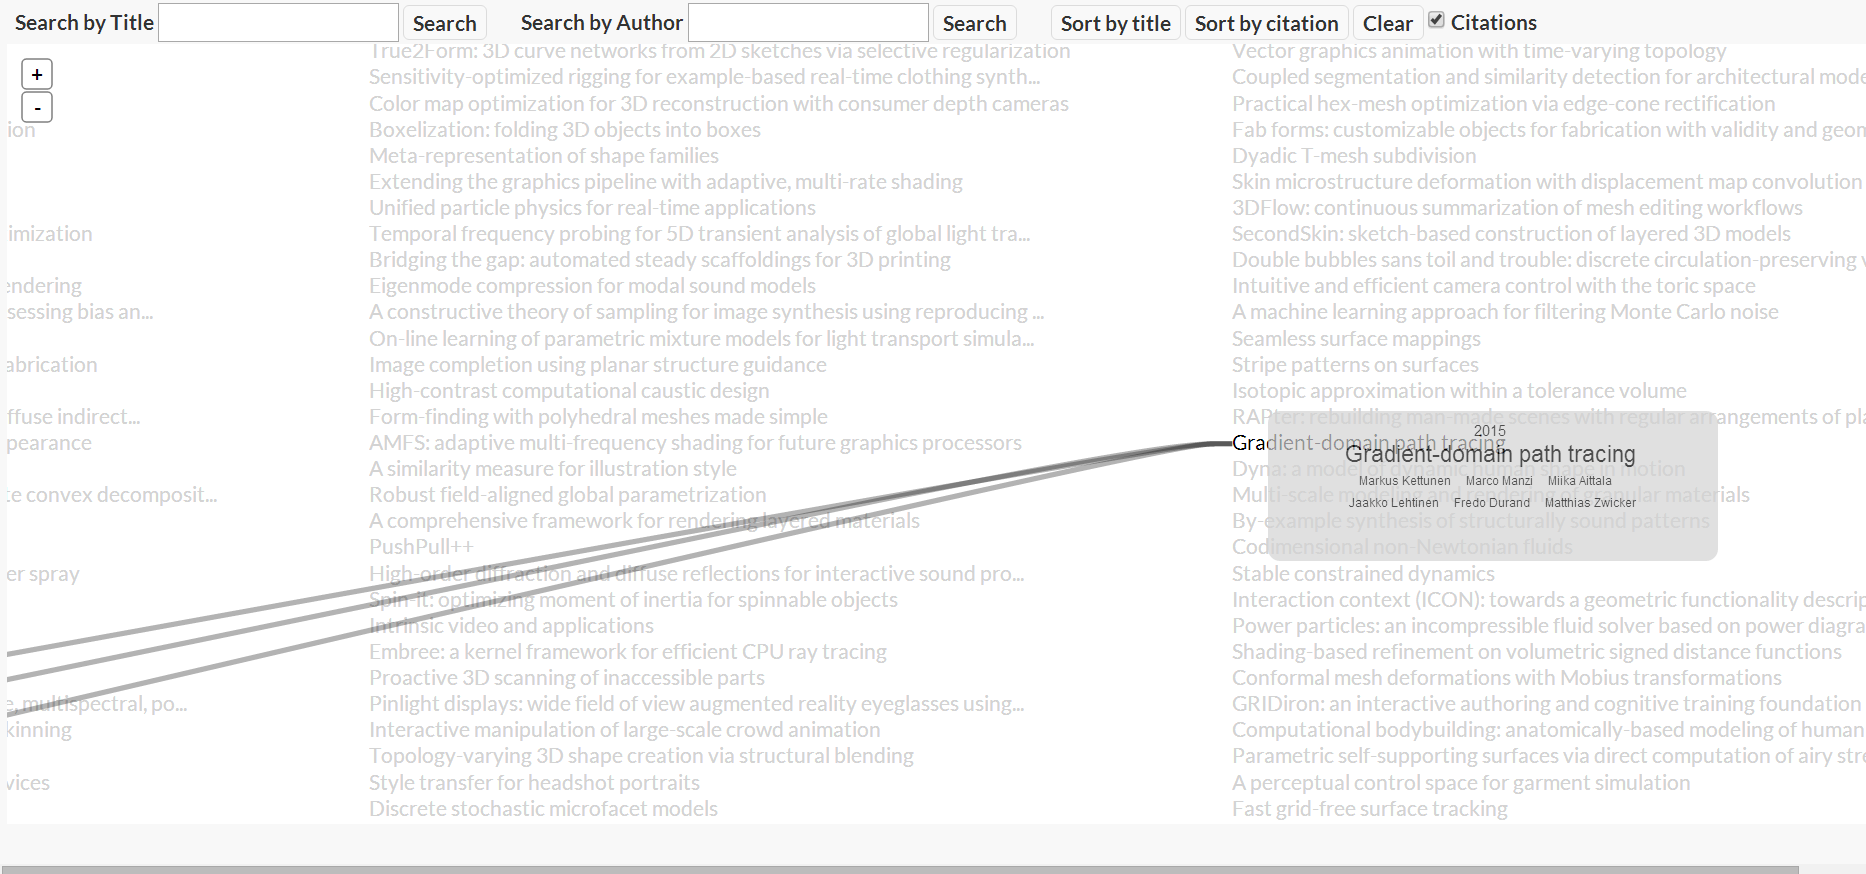
\includegraphics[width=0.7\textwidth]{gradient_domain_path_tracing.png}
    \caption{"Gradient domain path tracing" paper selected}
    \label{fig:gradient_domain_path_tracing_paper_selected}
\end{figure}

In the paper detail view, we can read the selected paper's abstract, as well as see a list of keywords associated with this paper (Figure \ref{fig:gradient_domain_path_tracing_paper_detail}).

\begin{figure}[ht]			
    \centering
    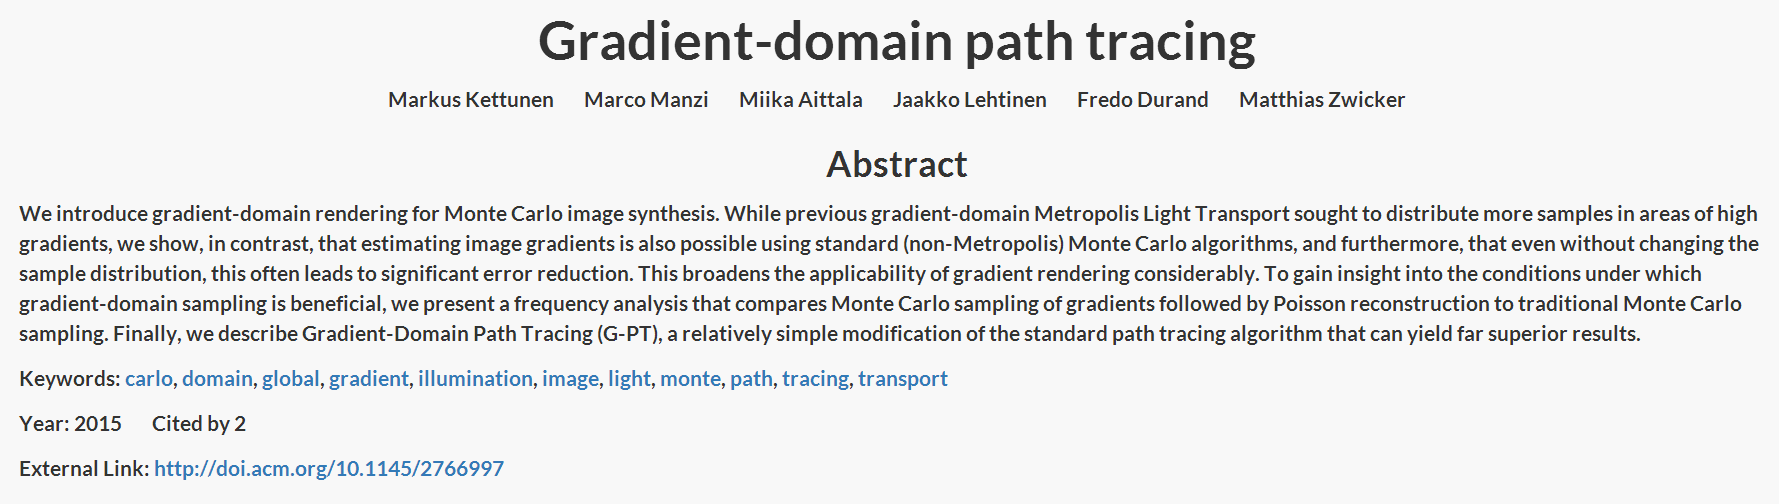
\includegraphics[width=0.7\textwidth]{gradient_domain_path_tracing_detail.png}
    \caption{"Gradient domain path tracing" paper abstract}
    \label{fig:gradient_domain_path_tracing_paper_detail}
\end{figure}

After reading the abstract and having a look at the keywords, we are interested in the keyword "path tracing", which is a technique to achieve global illumination. Clicking on these two words ("path" and "tracing") in the paper detail view bring us to the keyword view where these two keywords are selected (in addition to "global" and "illumination" which were selected before). Going back to the paper view, which now highlights all the papers with these four keywords. Looking at the recent years we notice there are two highlighted papers, one of which is the one that we have already seen (Figure \ref{fig:global_illumination_path_tracing_papers}).

\begin{figure}[ht]			
    \centering
    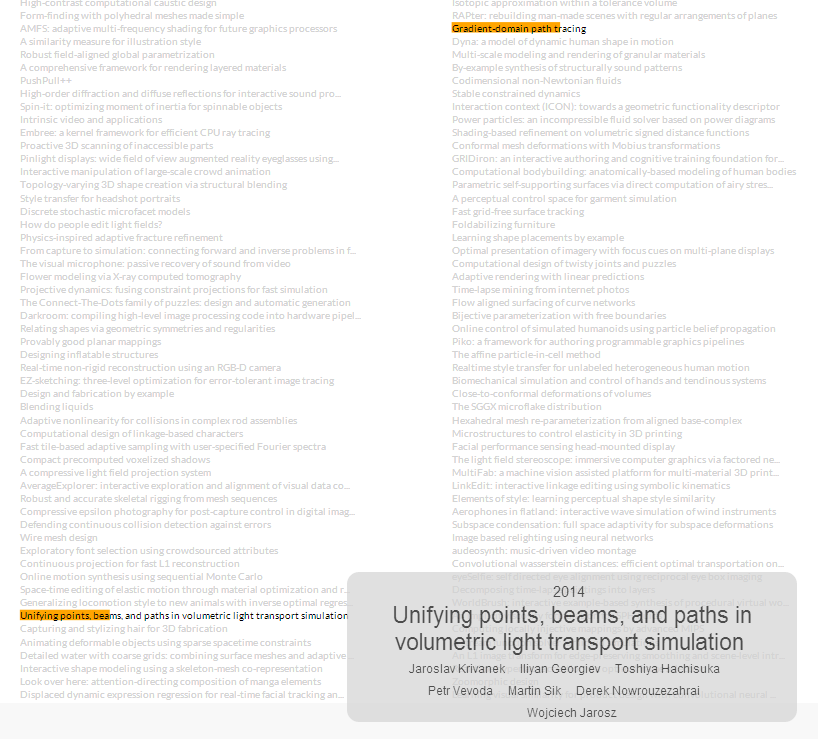
\includegraphics[width=0.7\textwidth]{global_illumination_path_tracing_papers.png}
    \caption{Papers having the four keywords "global", "illumination", "path" and "tracing"}
    \label{fig:global_illumination_path_tracing_papers}
\end{figure}

We click on the the other paper which is titled "Unifying points, beams, and paths in volumetric light transport simulation". After going to the paper detail view to read its abstract, we are interested in this paper and want to find papers that are related to it. We go back to the paper view and see that this paper references another paper in the same year, with a title that seems like it could be of interest to us: "Multiplexed metropolis light transport" (Figure \ref{fig:multiplexed_metropolis_light_transport_referenced}).

\begin{figure}[ht]			
    \centering
    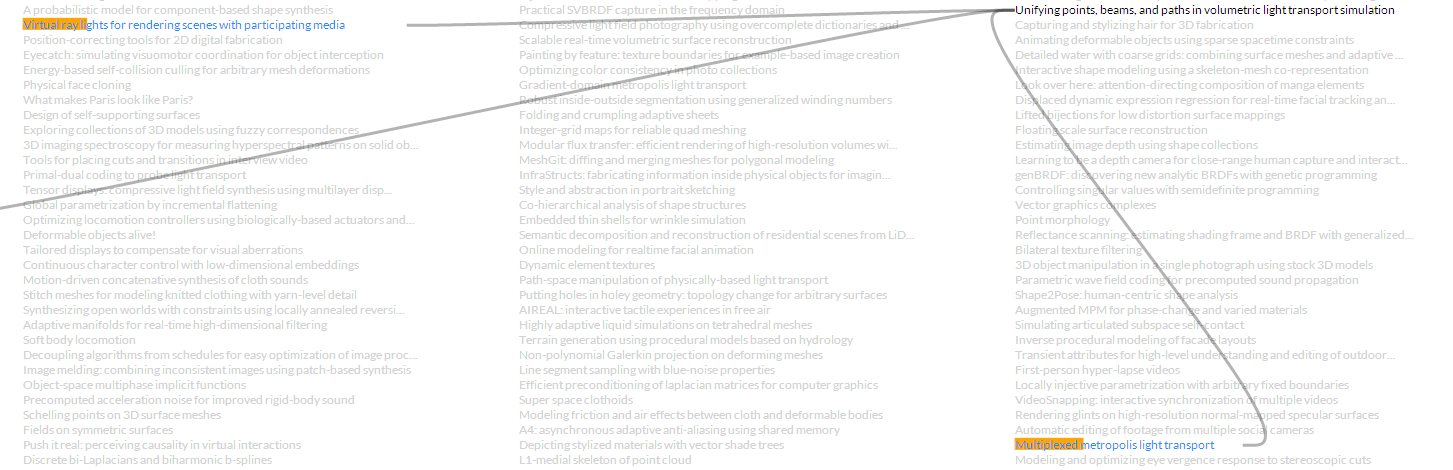
\includegraphics[width=0.7\textwidth]{multiplexed_metropolis_light_trasnport_referenced.png}
    \caption{Papers that our paper of interest references}
    \label{fig:multiplexed_metropolis_light_transport_referenced}
\end{figure}

Clicking on the paper "Multiplexed metropolis light transport", we can read its abstract and furthermore look at its authors. We notice that one of its authors, Carsten Dachsbacher, has written a paper in SIGGRAPH 2007 about a method that addresses the problem of "interactive global illumination" (the paper's title is "Implicit visibility and antiradiance for interactive global illumination") (Figure \ref{fig:carsten_dachsbacher}. We are interested in knowing more about this paper because unlike path tracing, which is a general but very slow solution to the problem of global illumination, this paper seems to propose a method that can compute global illumination at interactive rates.

\begin{figure}[ht]			
    \centering
    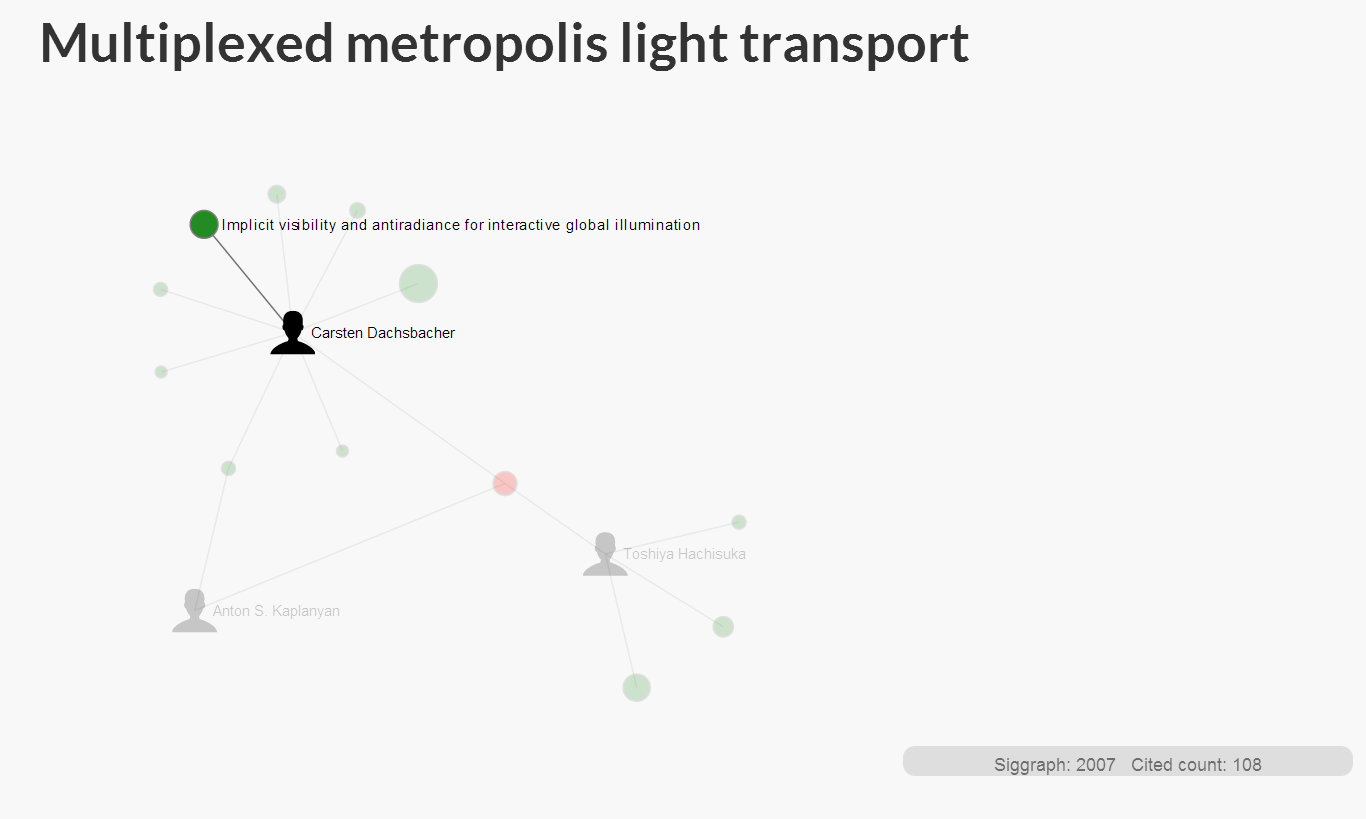
\includegraphics[width=0.7\textwidth]{carsten_dachsbacher.png}
    \caption{Carsten Dachsbacher's SIGGRAPH publications}
    \label{fig:carsten_dachsbacher}
\end{figure}

We then click on the paper "Implicit visibility and antiradiance for interactive global illumination" in the author view to select it. Back to the paper detail view we can read this paper's abstract and look at the list of papers that it references (Figure \ref{fig:antiradiance}). And from this we can continue our exploration of the space of papers that try to solve the global illumination problem in one way or another.

\begin{figure}[ht]			
    \centering
    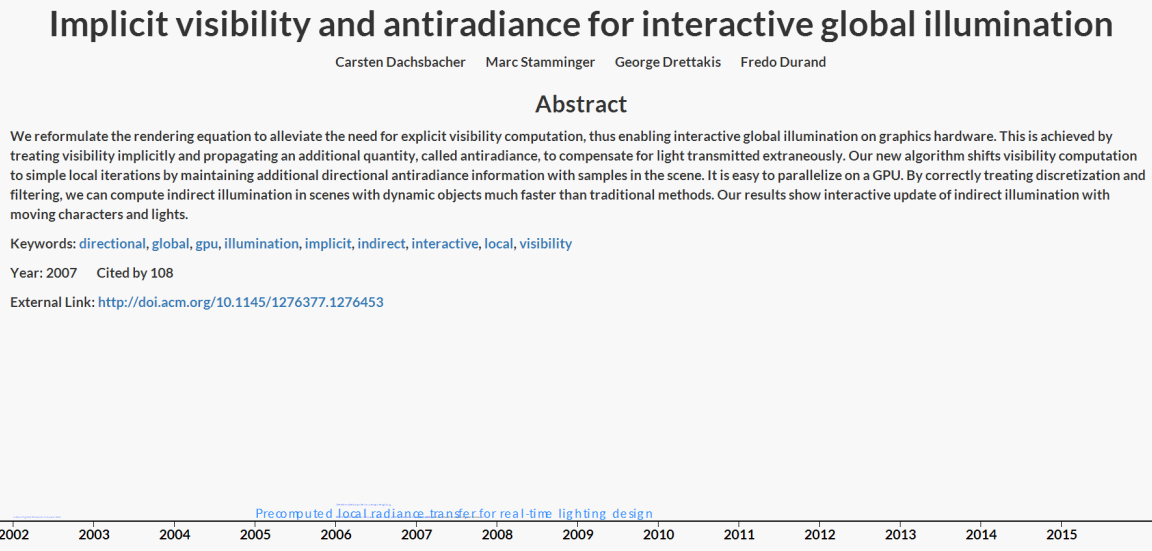
\includegraphics[width=0.7\textwidth]{antiradiance_paper_detail.png}
    \caption{Antiradiance paper details}
    \label{fig:antiradiance}
\end{figure}

\textbf{Conclusion}
We have shown that our tool provides several ways to navigate the space of papers that are related to certain topics of interest. One can use either the reference relationships, the common keyword relationships, or the common author relationships to get to the papers of interest and read their abstract to understand them more. On our way of exploring the data, we also  learn more about the various techniques employed and get an idea about who publish frequently in this topic. All of these can work together to help the user quickly get a high-level understanding of the field of research he or she is interested in.

\end{document}